\documentclass[../main.tex]{subfiles}
\begin{document}
\chapter{Fundamentos sobre funções}\label{cap_funcao}\index{Função}
\minitoc
%\tableofcontents
\subsection*{Objetivos de aprendizagem do capítulo}
\addcontentsline{toc}{section}{Objetivos de aprendizagem do capítulo}
Ao final deste capítulo você deverá ser capaz de:
\begin{itemize}
    \item Determinar com precisão o domínio e a imagem de uma função real;
    \item Classificar funções de diferentes categorias;
    \item Calcular o coeficiente angular da reta que determina uma função afim;
    \item Encontrar a expressão algébrica de uma função afim, dados dois pontos ou o coeficiente angular da reta correspondente e um de seus pontos;
    \item Traçar gráficos de funções afim, quadrática, exponencial, logarítmica e trigonométricas;
    \item Calcular raízes, coordenadas do vértice e soma e produto de raízes de uma função quadrática
    \item Diferenciar funções seno, cosseno, tangente, cotangente, secante e cossecante e identificar os gráficos correspondentes a cada uma delas;
    \item Manipular as identidades trigonométricas para encontrar outras equivalentes;
    \item Classificar as funções em crescente ou decrescente e em pares ou ímpares;
    \item Dada uma função, saber estabelecer se ela é injetora, sobrejetora ou bijetora;
    \item Realizar operações com funções, isto é, soma, substração, produto, divisão e composição de funções;
    \item Encontrar a inversa de uma função, se ela existir;
    \item Relacionar-se cada vez mais com a linguagem e o simbolismo matemático relativo às funções definidas no conjunto dos números reais.
\end{itemize}
\section{Introdução}
%Ao relacionarmos o espaço em função do tempo, a intensidade da fotossíntese realizada por uma planta em função da intensidade da luz a que ela é exposta, ou uma pessoa em função da impressão digital, percebemos quão importante é o conceito de função, pois este nos permite compreender as relações entre os fenômenos físicos, biológicos, sociais, etc., presentes no nosso cotidiano. Portanto, neste capítulo, revisaremos um dos conceitos mais importante da Matemática: a função. Iniciaremos o capítulo dando a definição formal deste objeto matemático, que é o objetivo de estudo deste capítulo e de todos os outros.

Em diversas situações, apresentam-se relações que existem entre um conjunto de objetos e outro conjunto de outros objetos, por exemplo: quando calculamos a área de um círculo, esta depende do raio do círculo; a distância de um objeto que viaja a uma velocidade constante ao longo de um percurso depende do tempo; etc. Em cada caso, o valor da quantidade variável, denotada por \(y\), depende do valor de outra quantidade variável, denotada por \(x\). Dizemos então que \(y\) é uma função de \(x\) e a escrevemos como \(y=f(x)\).


\begin{framed}
\begin{definition}
Sejam \(A\) e \(B\) dois conjuntos não vazios. Uma função \(f\) de \(A\) em \(B\), denotada por \(f:A\rightarrow B\), é uma regra que associa um único elemento \(f(x)\in B\) a cada elemento \(x\in A\).
\\ Costumeiramente, identificamos uma função por uma letra, por exemplo, $f$ e escrevemos $f:A\to B$, $y=f(x)$, para denotar que a função $f$ toma valores de entrada em $A$ e de saída em $B$.
\end{definition}
\end{framed}

O conjunto $A$ de todos os possíveis valores de entrada da função é chamado de \textbf{domínio}\index{Função!domínio}. O conjunto $B$ é denominado \textbf{contradomínio}\index{Função!contradomínio} e o conjunto de todos os valores $f(x)$ tal que $x\in A$ é chamado de \textbf{imagem}\index{Função!imagem} da função.

\nota{
Seja uma função \(f:A\rightarrow B\).
\begin{compactenum}[a.]
\item A notação \(y=f(x)\) (leia-se ``\(y\) é igual a \(f\) de \(x\)'') expressa que \(y\) é o valor de \(f\) em \(x\), neste caso, \(x\) é denominada variável independente e \(y\) variável dependente.
\item Se \(A\) e \(B\) são subconjuntos de \(\mathbb{R}\), então \(f\) é chamada de função real de variável real.
\item Os valores de \(x\) para os quais \(f(x)=0\) são as coordenadas \(x\), para os quais o gráfico de \(f\) intersecta o eixo \(x\). Estes valores são denominados zeros de \(f\), raízes de \(f(x)=0\) ou pontos de corte de \(y=f(x)\) com o eixo \(x\).
%\item Os gráficos podem fornecer uma informação visual importante sobre uma função. Por exemplo, como o gráfico de uma função \(f\) no plano \(xy\) é o gráfico da equação \(y=f(x)\). Os pontos do gráfico são da forma \((x,f(x))\), ou seja, a coordenada \(y\) de um ponto do gráfico de \(f\) é o valor de \(f\) na coordenada \(x\) correspondente.
\end{compactenum}

}

\begin{ex}
Para \(f\) definida a seguir, determinemos o domínio e imagem:
\begin{compactenum}[a)]
\item Sejam \(A=\{1,2,3,4\}\), \(B=\{5,6,7,8,9\}\) e \(f:A\rightarrow B\) definida por \(f(x)=x+2\).\\
\begin{solution}
Desde que \(f({\bf 1})={\bf 1}+2=3\), \(f({\bf 2})={\bf 2}+2=4\), \(f({\bf 3})={\bf 3}+2=5\), \(f({\bf 4})={\bf 4}+2=6\), verificamos que os únicos valores de \(A\) que tem um correspondente no conjunto \(B\) são \(3,\,\,\,4\). Portanto, \({\rm Dom}(f)=\{3,4\}\) e \({\rm Im}(f)=\{5,6\}\).
\end{solution}
\item Seja \(f:\mathbb{R}\rightarrow \mathbb{R}\) definida por \(f(x)=\dfrac{1}{x}\).\\
\begin{solution}
A função \(f\) dada está definida para todo \(x\in \mathbb{R}\), exceto \(x=0\); assim \({\rm Dom}(f)=\mathbb{R}\setminus\{0\}\).
Para determinar \({\rm Im}(f)\) é conveniente introduzir uma variável dependente \(y\):

\[y=\dfrac{1}{x}.\]
Embora para muitos o conjunto dos possíveis valores de \(y\) não seja evidente nessa equação, o gráfico de \(f\) sugere que \({\rm Im}(f)=\mathbb{R}\setminus\{0\}\). Para provar isto, resolvamos a equação acima para \(x\), em termos de \(y\):

\[x\neq 0\quad\Rightarrow\quad xy=1\quad\Leftrightarrow\quad x=\dfrac{1}{y}.\]
Agora está evidente que essa expressão está definida para todo \(y\in \mathbb{R}\), exceto para \(y=0\). Portanto, \({\rm Im}(f)=\mathbb{R}\setminus\{0\}\).
\end{solution}
\item Seja \(f:(0,5]\to [1,10)\) definida por \(f(x)=(x-3)^2 +1\).\\
\begin{solution}
Da definição de \(f\) temos que, para qualquer valor de $(0, 5]$ está bem definida. Assim, \({\rm Dom}(f)=(0,5]\). Por outro lado, para \(x \in (0,5]\), se segue que

\[0<x\leq 5\quad \Leftrightarrow\quad -3<x-3\leq 2 \quad \Leftrightarrow\quad 0\leq (x-3)^2<9\Leftrightarrow\quad 1\leq (x-3)^2+1<10\]
Logo, o valor de \(f(x)\) varia sobre o intervalo \([1,10)\). Portanto, \({\rm Im}(f)=[1,10)\).

Nesse caso, \(f\) é uma aplicação de \((0,5]\) sobre \([1,10)\) e \({\rm Im}(f)\) pode ser escrita como \(f((0,5])=[1,10)\). 
\end{solution}
\end{compactenum}
\end{ex}

\begin{ex}
  Determinemos o domínio e a imagem de cada uma das seguintes funções:
  \begin{itemize}
  \item $y=x^2$:
    \begin{itemize}
    \item Para qualquer número real $x$, temos que $x^2$ também é um número real. Então, dizemos que seu domínio (natural)\footnote{O \textbf{domínio natural}\index{Função!domínio natural} é o conjunto de todos os números reais tais que a expressão matemática que define a função seja possível.} é o conjunto $\mathbb{R} = (-\infty, \infty)$.
    \item Para cada número real $x$, temos $y=x^2\geq0$. Além disso, para cada número real não negativo $y$, temos que $x=\sqrt{y}$ é tal que $y=x^2$. Assim sendo, concluímos que a imagem da função é o conjunto de todos os números reais não negativos, i.e. $[0, \infty)$.
    \end{itemize}
  \item $y=1/x$:
    \begin{itemize}
    \item Lembremos que divisão por zeros não está definida. Logo, o domínio desta função é o conjunto dos números reais não nulos, i.e. $(-\infty, 0)\cup (0, \infty)$.
    \item Primeiramente, observemos que se $y=0$, então não existe número real tal que $0=1/x$. Ou seja, $0$ não pertence a imagem desta função. Por outro lado, dado qualquer número $y\neq 0$, temos que $x=1/y$ é tal que $y=1/x$. Logo, concluímos que a imagem desta função é o conjunto de todos os números reais não nulos, i.e. $(-\infty, 0)\cup (0, \infty)$.
    \end{itemize}
  \item $y=\sqrt{1-x^2}$:   
    \begin{itemize}
    \item Lembremos que a raiz quadrada de números negativos não está definida. Portanto, precisamos que:
      \begin{align*}
        1-x^2\geq 0 &\Rightarrow x^2 \leq 1\\
                    &\Rightarrow -1 \leq x \leq 1
      \end{align*}
      Donde concluímos que o domínio desta função é o conjunto de todos os números $x$ tal que $-1\leq x \leq 1$ (ou, equivalentemente, o intervalo $[-1, 1]$).
      
      
 No \geogebra~ digite $1-x^2\geq $ que ele fornece graficamente o intervalo de definição do domínio da função.
\    \item Uma vez que $-1 \leq x \leq 1$, temos que $0 \leq 1-x^2 \leq 1$ e, portanto, $0\leq \sqrt{1-x^2} \leq 1$. Ou seja, a imagem desta função é o intervalo $[0, 1]$.
    \end{itemize}
  \end{itemize}
\end{ex}

\section{Gráficos de funções}\index{Função!gráfico}\label{sec:GrafFunc}
O \textbf{gráfico}\index{gráfico} de uma função é o conjunto dos pares ordenados $(x, f(x))$ tal que $x$ pertence ao domínio da função. Mais especificamente, para uma função $f:A\to \mathbb{R}$, o gráfico é o conjunto
\begin{equation}
  \{(x, f(x))| x\in A\}.
\end{equation}

O \textbf{esboço do gráfico}\index{gráfico} de uma função é, costumeiramente, uma representação geométrica dos pontos de seu gráfico em um plano cartesiano\index{plano cartesiano}.

\begin{ex}\label{ex:grafico}
  A Figura \ref{fig:ex_grafico} mostra os esboços dos gráficos das funções $f(x)=x^2$, $g(x)=1/x$ e $h(x)=\sqrt{1-x^2}$.
  
  \begin{figure}[H]
    \centering
    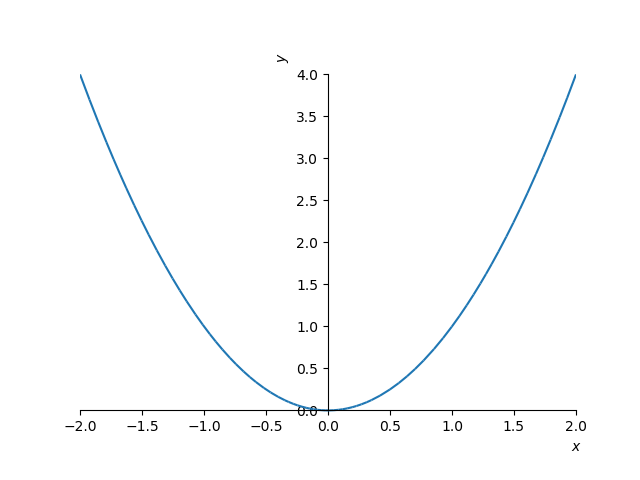
\includegraphics[width=0.3\textwidth]{fig_func/fig_ex_grafico_x2}~
    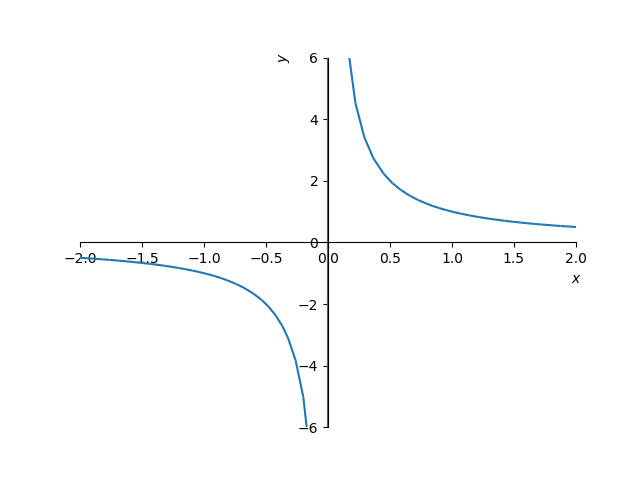
\includegraphics[width=0.3\textwidth]{fig_func/fig_ex_grafico_1x}~
    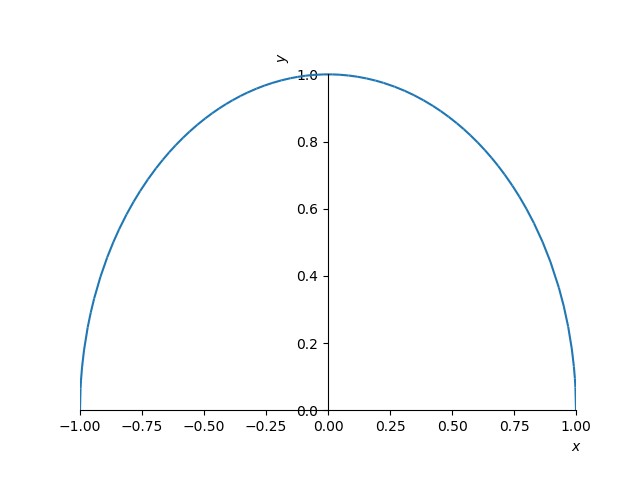
\includegraphics[width=0.3\textwidth]{fig_func/fig_ex_grafico_s1x2}
    \caption{Esboço dos gráficos das funções $f(x)=x^2$, $g(x)=1/x$ e $h(x)=\sqrt{1-x^2}$ dadas no Exemplo \ref{ex:grafico}.}
    \label{fig:ex_grafico}
  \end{figure}

  
 
 \dica Para plotarmos os gráficos destas funções no GeoGebra\index{GeoGebra} basta digitá-la na ordem desejada.
\end{ex}

\subsection{Exercícios resolvidos}
\begin{exeresol}\label{exeresol:funpot_graf}
  Determine o domínio e faça um esboço do gráfico de cada uma das seguintes funções:\\
$\displaystyle f(x) = x^{5/2}$\hfill  $\displaystyle f(x) = x^{5/3}$\\
\begin{resol}
 \noindent\begin{enumerate}[a)]
  \item Vamos analisar a função $f(x) = x^{5/2}$. Como $x^{5/2} = \sqrt{x^5}$ e não existe a raiz quadrada de número negativo, temos que $x^5$ deve ser não negativo. Daí, $x$ deve ser não negativo. Logo, o domínio de $f(x) = x^{5/2}$ é $[0, \infty)$. Veja o esboço desta função na Figura \ref{fig:exeresol_funpot_graf_a}.

    \begin{figure}[H]
      \centering
      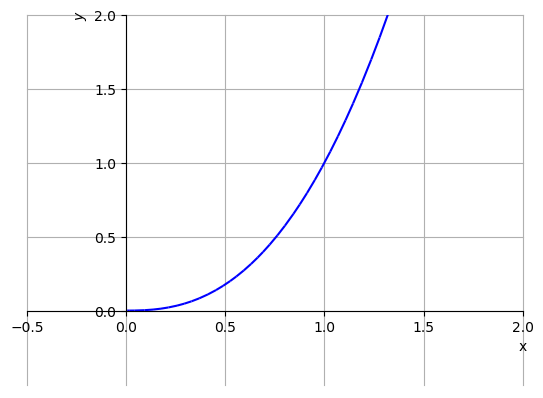
\includegraphics[width=0.5\textwidth]{fig_func/fig_exeresol_funpot_graf_a}
      \caption{Esboço do gráfico de $f(x) = x^{5/2}$.}
      \label{fig:exeresol_funpot_graf_a}
    \end{figure}

    
    Para plotar o gráfico de $f(x)$ no \geogebra, basta digitar a função da seguinte maneira: \verb|f(x)=x^(5/2)|
  \item Vamos analisar a função $g(x) = x^{5/3}$. Como $x^{5/3} = \sqrt[3]{x^5}$, não temos restrição sobre os valores de $x$. Logo, o domínio da função $g$ é $(-\infty, \infty)$. Veja o esboço desta função na Figura \ref{fig:exeresol_funpot_graf_b}.

    \begin{figure}[H]
      \centering
      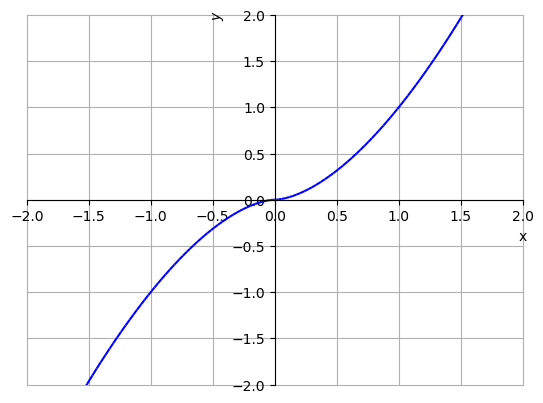
\includegraphics[width=0.5\textwidth]{fig_func/fig_exeresol_funpot_graf_b}
      \caption{Esboço do gráfico de $g(x) = x^{5/3}$.}
      \label{fig:exeresol_funpot_graf_b}
    \end{figure}


    Para plotar o gráfico de $g(x)$ no \geogebra, digitamos: \verb|f(x)=x^(5/3)|
   \end{enumerate}
\end{resol}
\end{exeresol}

\subsection{Exercícios}
\begin{exer}
  Determine o domínio, a imagem e faça um esboço do gráfico de cada uma das seguintes funções:
  \begin{enumerate}[a)]
  \item $f(x) = x^7$
  \item $g(x) = x^8$
  \end{enumerate}
\end{exer}
\begin{resp}
  a) domínio: $(-\infty, \infty)$; imagem: $(-\infty, \infty)$. b) domínio: $(-\infty, \infty)$; imagem: $[0, \infty)$. Dica: use o \href{https://www.geogebra.org/graphing}{GeoGebra} para verificar os esboços de seus gráficos.
\end{resp}

\begin{exer}
  Determine o domínio e a imagem da função identidade, i.e. $f(x) = x$
\end{exer}
\begin{resp}
  Domínio: $(-\infty, \infty)$; Imagem: $(-\infty, \infty)$
\end{resp}

\begin{exer}
  Determine o domínio e a imagem da função $f(x) = x^2 + 1$
\end{exer}
\begin{resp}
  Domínio: $(-\infty, \infty)$; Imagem: $[1, \infty)$
\end{resp}

\begin{exer}
  Determine o domínio e a imagem da função
  \begin{equation*}
    h(x) = \frac{1}{x-1} - 2
  \end{equation*}
\end{exer}
\begin{resp}
  Domínio: $(-\infty, 1)\cup (1, \infty)$; Imagem: $(-\infty, -2)\cup (-2, \infty)$
\end{resp}
\begin{exer}
  Determine o domínio, a imagem e faça um esboço do gráfico de cada uma das seguintes funções:
  \begin{enumerate}[a)]
  \item $\displaystyle f(x) = \frac{1}{x^7}$
  \item $\displaystyle g(x) = \frac{1}{x^8}$
  \end{enumerate}
\end{exer}
\begin{resp}
  a) domínio: $(-\infty, \infty)\setminus\{0\}$; imagem: $(-\infty, \infty)\setminus\{0\}$. b) domínio: $(-\infty, \infty)\setminus\{0\}$; imagem: $(0, \infty)$. Dica: use o \href{https://www.geogebra.org/graphing}{GeoGebra} para verificar os esboços de seus gráficos.
\end{resp}

\begin{exer}
  Determine o domínio, a imagem e faça um esboço do gráfico de cada uma das seguintes funções:
  \begin{enumerate}[a)]
  \item $\displaystyle f(x) = \sqrt{x^2}$
  \item $\displaystyle g(x) = \sqrt[3]{x^3}$
  \end{enumerate}
\end{exer}
\begin{resp}
  a) domínio: $(-\infty, \infty)$; imagem: $[0, \infty)$. b) domínio: $(-\infty, \infty)$; imagem: $(-\infty, \infty)$. Dica: use o \href{https://www.geogebra.org/graphing}{GeoGebra} para verificar os esboços de seus gráficos.
\end{resp}

\section{Categorizações de funções}
\subsection{Funções algébricas}\index{Função!algébricas}

{\bf Funções algébricas}\index{Função!!algébrica} são funções definidas a partir de somas, subtrações, multiplicações, divisões ou extração de raízes de funções polinomiais. Estudaremos estas funções ao longo do curso de cálculo.
\subsection{Funções transcendentes}\index{Função!transcendentes}

{\bf Funções transcendentes}{\index{Função!!transcendente}} são funções que não são algébricas. Como exemplos, temos as funções trigonométricas, exponencial e logarítmica, as quais introduziremos nas próximas seções.
\subsection{Funções definidas por partes}\index{Função!por partes}

\textbf{Funções definidas por partes}\index{Função!!partes} são funções definidas por diferentes expressões matemáticas em diferentes partes de seu domínio.

Um exemplo fundamental de função definida por partes é a \textbf{função valor absoluto}\footnote{Esta função também pode ser definida por $|x| = \sqrt{x^2}$.}
\begin{equation}
  |x| = \left\{
    \begin{array}{ll}
      x, & x\leq 0\\
      -x, & x<0
    \end{array}
\right.
\end{equation}
Vejamos o esboço do seu gráfico dado na Figura \ref{fig:cap_funcao_funabs}.

\begin{figure}[!htb]
  \centering
  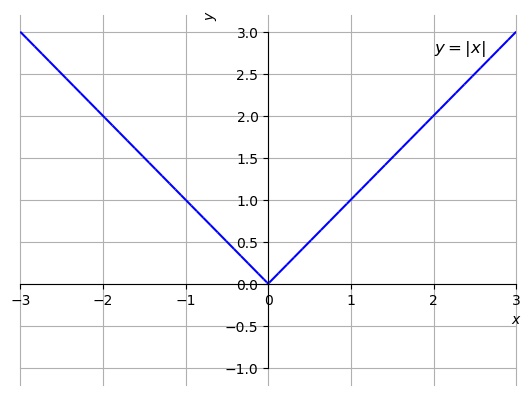
\includegraphics[width=0.5\textwidth]{fig_func/fig_cap_funcao_funabs}
  \caption{Esboço do gráfico da função valor absoluto $y=|x|$.}
  \label{fig:cap_funcao_funabs}
\end{figure}

\section{Função polinomial}\label{sec:FuncPolinomiais}

Uma {\bf função polinomial}\index{Função! polinomial} ({\bf polinômio}\index{polinômio}) tem a forma
\begin{equation}
  p(x) = a_nx^n + a_{n-1}x^{n-1} + \cdots + a_1x + a_0
\end{equation}
onde $a_i$ são coeficientes reais, $a_n\neq 0$ e $n$ é inteiro não negativo, este chamado de {\bf grau do polinômio}\index{grau do polinômio}.

Polinômios são definidos em toda parte\footnote{Uma função é dita ser definida em toda parte quando seu domínio é $(\infty, \infty)$}. Polinômios de grau ímpar tem imagem $(-\infty, \infty)$. Entretanto, a imagem polinômios de grau par dependem de cada caso. Iremos estudar mais propriedades de polinômios ao longo do curso de cálculo. Veja a Figura \ref{fig:poli_graficos}.
\begin{figure}[H]
  \centering
  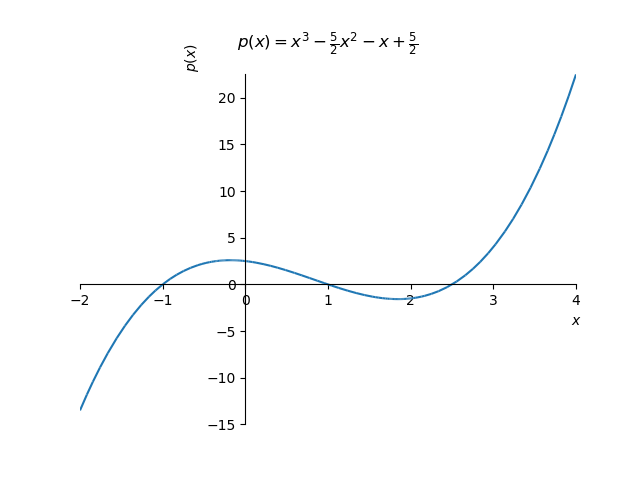
\includegraphics[width=0.5\textwidth]{fig_func/fig_poli_impar}~
    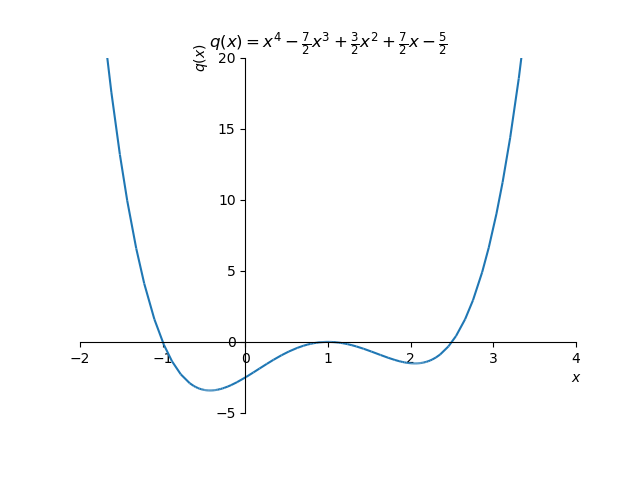
\includegraphics[width=0.5\textwidth]{fig_func/fig_poli_par}
  \caption{Esboços dos gráficos das funções polinomiais. Esquerda $p(x) = x^{3} - 2.5 x^{2} - 1.0 x + 2.5$. Direita: $q(x) = x^{4} - 3.5 x^{3} + 1.5 x^{2} + 3.5 x - 2.5$.}
  \label{fig:poli_graficos}
\end{figure}

Quando $n=0$, temos um polinômio de grau 0 (ou uma função constante). Quando $n=1$, temos um polinômio de grau 1 (ou, uma função afim). Ainda, quando $n=2$ temos uma {\bf função quadrática}\index{Função!!quadrática} (ou {\bf polinômio quadrático}\index{polinômio!quadrático}) e, quando $n=3$, temos uma {\bf função cúbica}\index{Função!!cúbica} (ou {\bf polinômio cúbico}\index{polinômio cúbico}).

\section{Função afim}\index{Função!afim}\label{sec:FuncAfim}
\subsection{Definição e Exemplos}\index{Função afim!definição e exemplos}
Uma \textbf{função afim} é uma função da forma
\begin{equation}
f(x) = mx + b
\end{equation}
sendo $m$ e $b$ parâmetros  dados. O parâmetro $m$ é chamado de \textbf{coeficiente angular}\index{Funçao afim!coeficiente} e o parâmetro $b$ é chamado de \textbf{coeficiente constante} ou \textbf{coeficiente linear}.

Quando $m=0$, temos uma \textbf{função constante}\index{Função!constante} $f(x) = b$. Esta tem domínio $(-\infty, \infty)$ e imagem $\{b\}$. 

 Quando $b=0$ e $m\neq 0$, temos uma \textbf{função linear}\index{Função!linear} $f(x)=mx$, cujo domínio é $(-\infty, \infty)$ e imagem é $(-\infty, \infty)$. 
 
 Quando $m=1$ e $b=0$, a função afim é chamada de função identidade\index{Função!identidade}. Neste caso, qualquer que seja $x$ pertencente ao domínio da função, temos que $f(x)=x$.

O lugar geométrico do gráfico de uma função afim é uma \textbf{reta}\index{reta} (ou linha). O \textbf{coeficiente angular} \emph{$m$} controla a inclinação da reta em relação ao eixo $x$. Quando $m=0$, temos uma reta horizontal. \red{Quando $m>0$ temos uma reta com inclinação positiva (crescente) e, quando $m<0$ temos uma reta com inclinação negativa}.\\

A inclinação de uma reta é, normalmente, medida pelo ângulo de declividade (veja a Figura \ref{fig:declividade}). Para definirmos este ângulo, sejam $(x_0, y_0)$ e $(x_1, y_1)$, $x_0<x_1$, pontos sobre uma dada reta, gráfico da função afim $f(x)=mx+b$. O ângulo de declividade (ou, simplesmente, a declividade) da reta é, por definição, o ângulo formado pelo segmento que parte de $(x_0, y_0)$ e termina em $(x_1, y_0)$ e o segmente que parte de $(x_0, y_0)$ e termina em $(x_1, y_1)$. Denotando este ângulo por $\theta$, temos
\begin{align*}
  \tg\theta &= \frac{y_1-y_0}{x_1-x_0}\\
            &= \frac{mx_1+b-(mx_0+b)}{x_1-x_0}\\
            &= m
\end{align*}
o que justifica chamar $m$ de coeficiente angular.
\begin{figure}[H]
  \centering
  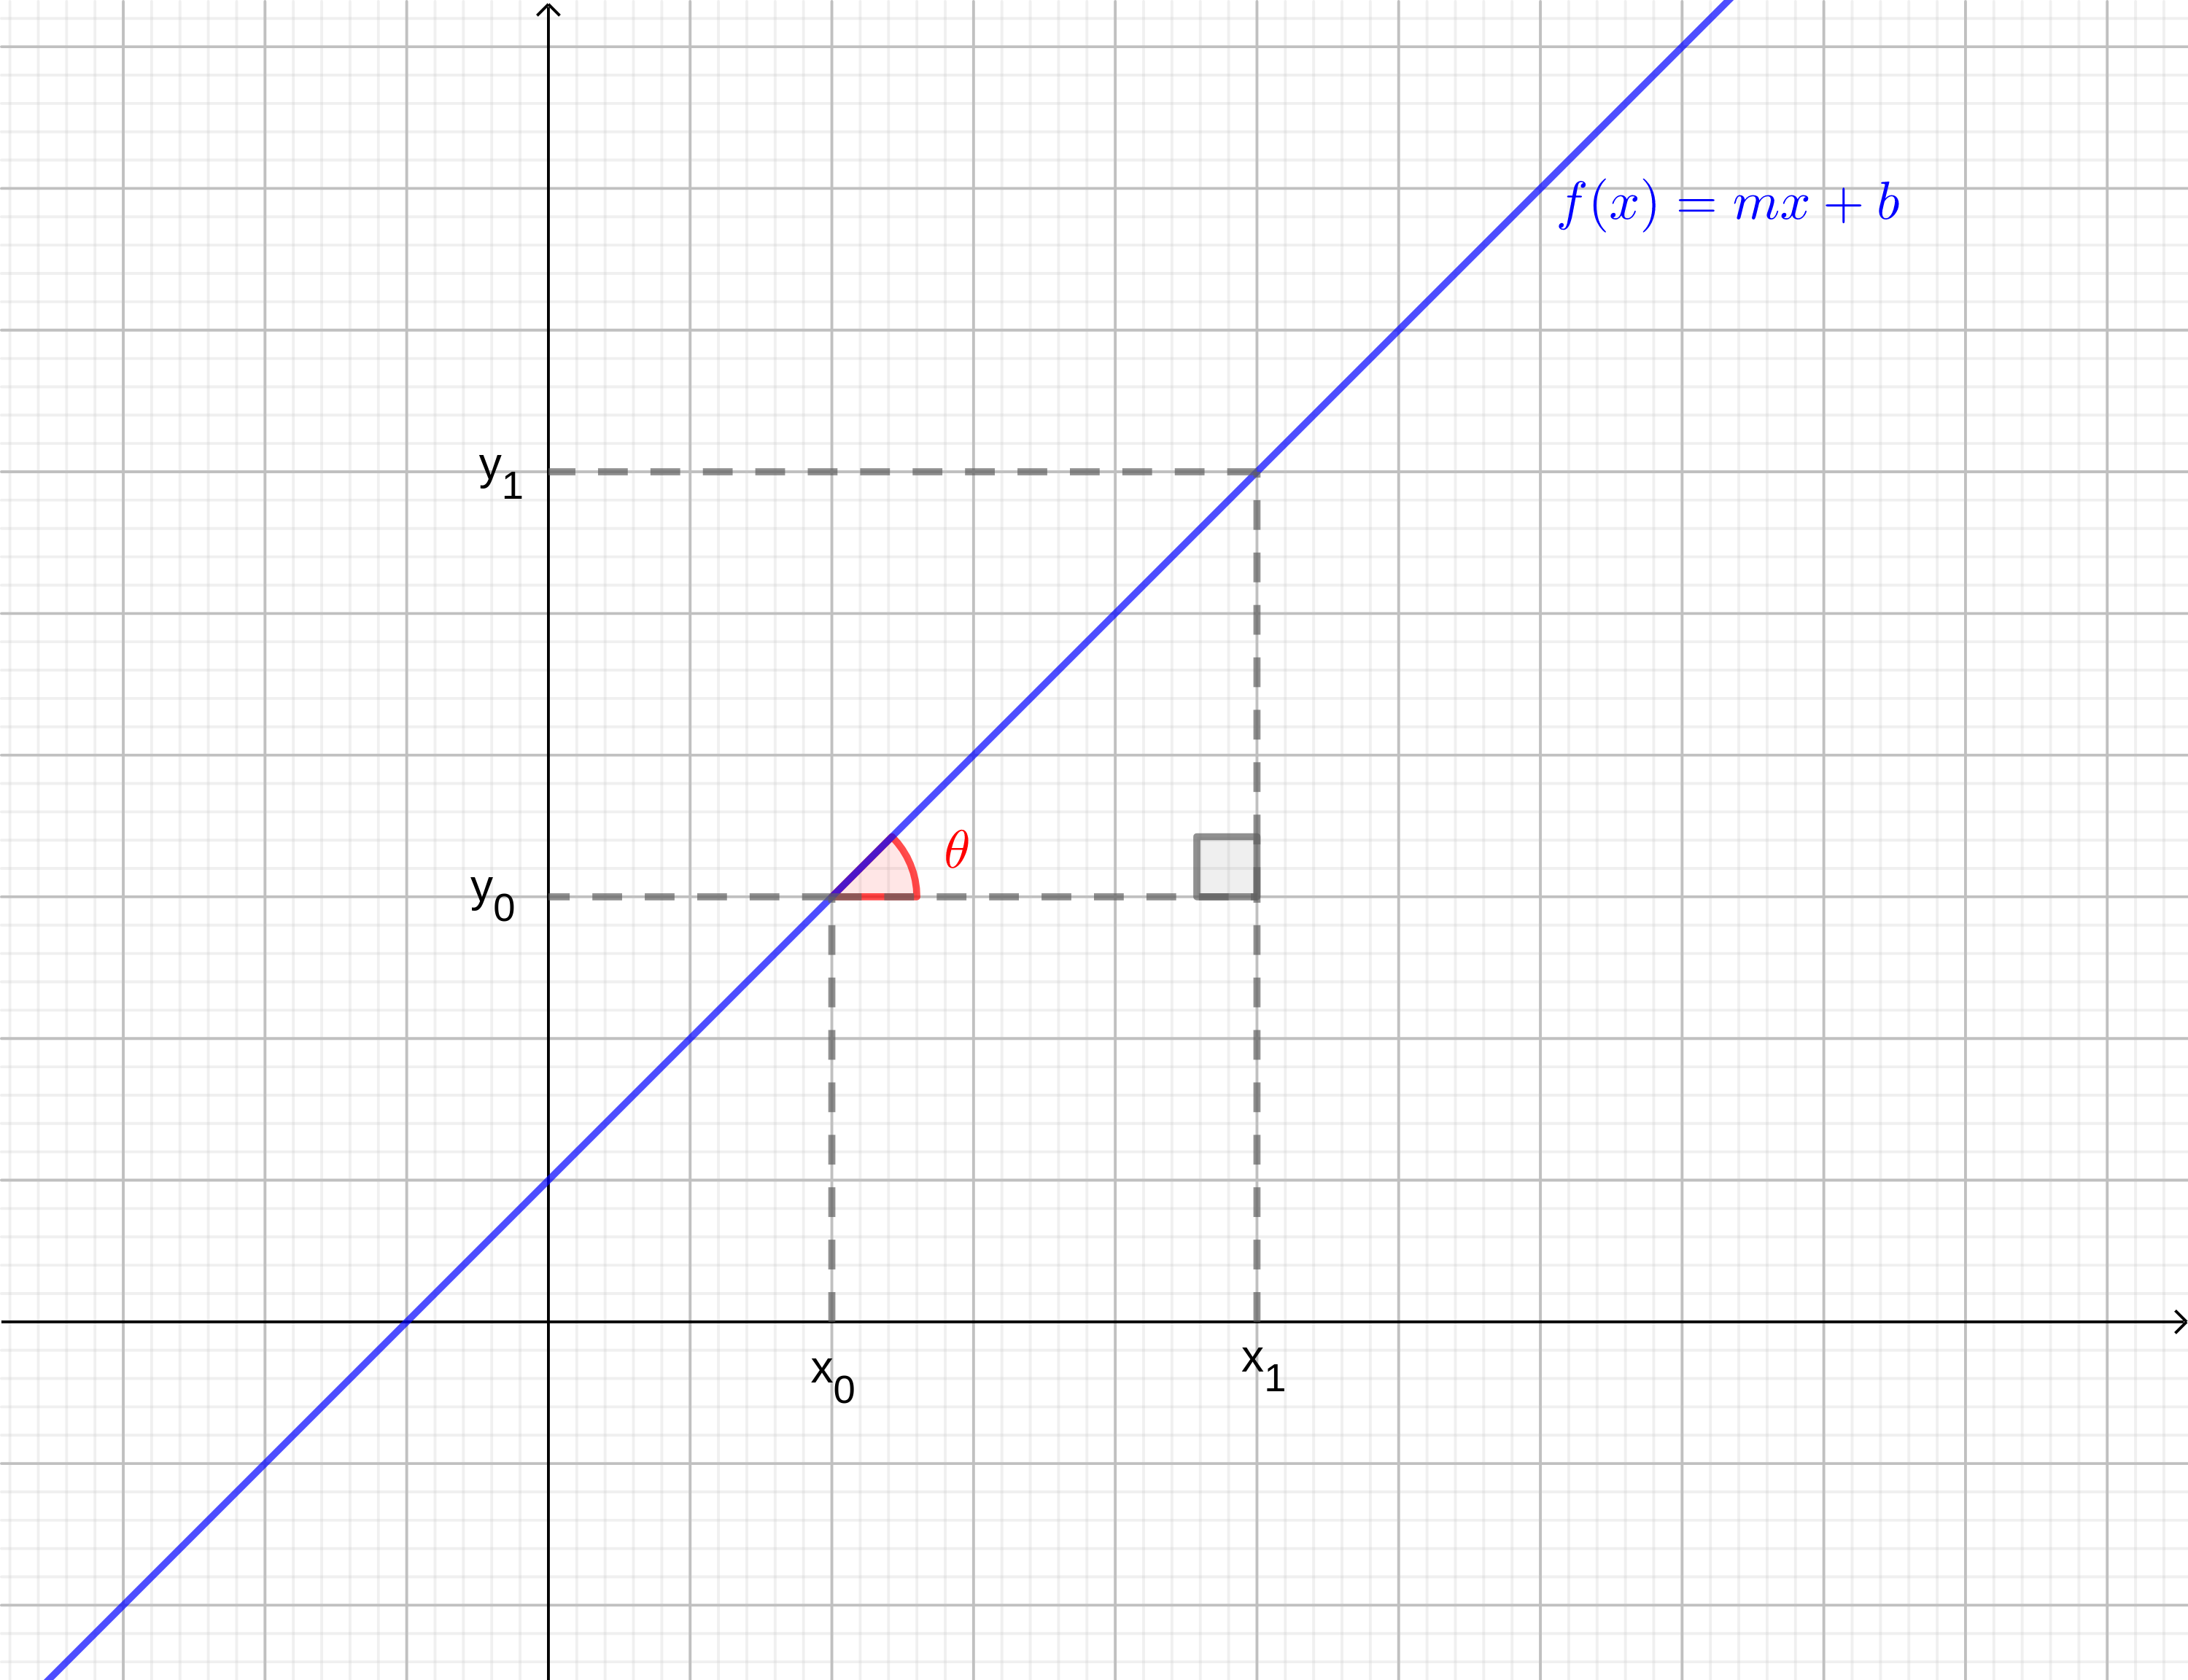
\includegraphics[width=0.55\textwidth]{fig_func/fig_declividade}
  \caption{Declividade e o coeficiente angular.}
  \label{fig:declividade}
\end{figure}

Quaisquer dois pontos $(x_0, y_0)$ e $(x_1, y_1)$, com $x_0\neq x_1$, determinam uma única função afim (reta) que passa por estes pontos. Para encontrar a expressão desta função, basta resolver o seguinte sistema linear
\begin{align*}
  mx_0 + b &= y_0\\
  mx_1 + b &= y_1
\end{align*}
Subtraindo a primeira equação da segunda, obtemos
\begin{equation}
  m(x_0-x_1) = y_0-y_1 \Rightarrow \boldsymbol{m = \frac{y_0-y_1}{x_0-x_1}}
\end{equation}
Daí, substituindo o valor de $m$ na primeira equação do sistema, obtemos
\begin{equation*}
  \frac{y_0-y_1}{x_0-x_1}x_0 + b = y_0 \Rightarrow b = -\frac{y_0-y_1}{x_0-x_1}x_0 + y_0
\end{equation*}
Ou seja, a expressão da função linear (equação da reta) que passa pelos pontos $(x_0, y_0)$ e $(x_1, y_1)$ é
\begin{equation}\label{eq:funafim_eq}
 \boldsymbol{ y = \underbrace{\frac{y_0-y_1}{x_0-x_1}}_{m}(x-x_0) + y_0}
\end{equation}


\begin{ex}\label{ex:funafim}
  A Figura \ref{fig:ex_funafim} mostra esboços dos gráficos das funções afins $f(x)=-5/2$, $f(x)=2$ e $f(x)=2x-1$.
    \begin{figure}[H]
    \centering
    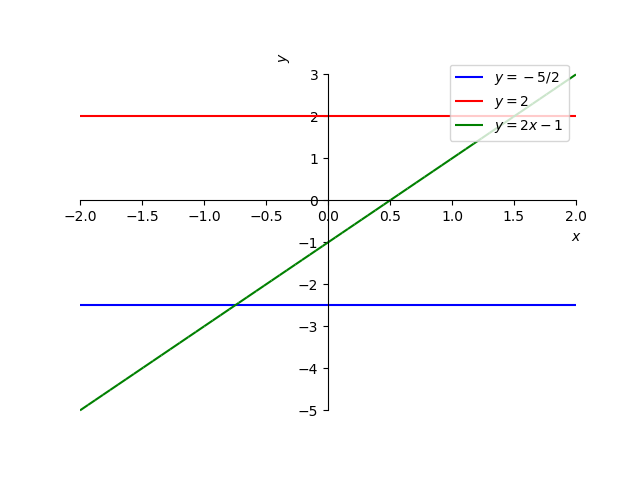
\includegraphics[width=0.65\textwidth]{fig_func/fig_ex_funafim}
    \caption{Esboços dos gráficos das funções afins $y=-5/2$, $y=2$ e $y=2x-1$ discutidas no Exemplo \ref{ex:funafim}.}
    \label{fig:ex_funafim}
  \end{figure}

{\normalfont \contour{red}{\color{white}\scshape Atenção:}}
\dica Faça o esboço destes gráficos no \geogebra.
\end{ex}

\begin{ex}\label{ex:funlinear}
  A Figura \ref{fig:ex_funlinear} mostra esboços dos gráficos das funções lineares $f_1(x)=\frac{1}{2}x$, $f_2(x) = x$, $f_3(x) = 2x$, $f_4(x)=-2x$, $f_5(x)=-x$ e $f_6(x)=-\frac{1}{2}x$
    \begin{figure}[H]
    \centering
    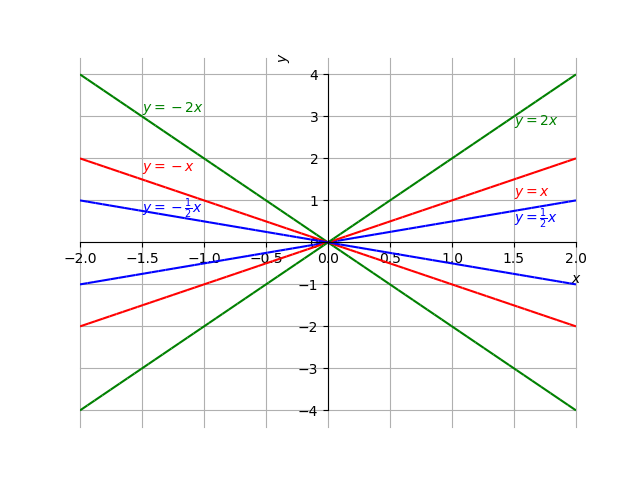
\includegraphics[width=0.7\textwidth]{fig_func/fig_ex_funlinear}
    \caption{Esboços dos gráficos das funções lineares discutidas no Exemplo \ref{ex:funlinear}.}
    \label{fig:ex_funlinear}
  \end{figure}
\end{ex}
\subsection{Exercícios resolvidos}\index{Exercícios resolvidos!Função afim}
\begin{exeresol}
Trace o esboço da reta que representa o gráfico da função afim $f(x) = -x-1$.\\  
\begin{resol}
  Para esboçar o gráfico de uma função afim, basta traçarmos a reta que passa por quaisquer dois pontos distintos de seu gráfico. Por exemplo, no caso da função $f(x) = -x -1$, temos
  \begin{center}
  \begin{tabular}[H]{r|c}
    $x$ & $y = -x-1$\\\hline
    -1  & 0\\
    1   & -2\\\hline
  \end{tabular}
\end{center}
Assim sendo, marcamos os pontos $(-1, 0)$ e $(1, -2)$ em um plano cartesiano e traçamos a reta que passa por eles. Veja a Figura \ref{fig:exeresol_funafim_grafico}.
\begin{figure}[htb]
  \centering
  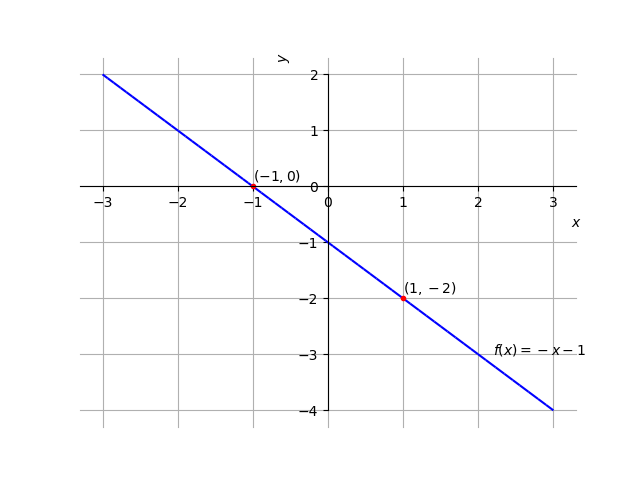
\includegraphics[width=0.65\textwidth]{fig_func/fig_exeresol_funafim_grafico}
  \caption{Esboço do gráfico da função afim $f(x)=-x-1$.}
  \label{fig:exeresol_funafim_grafico}
\end{figure}

\dica No \geogebra~ plote o gráfico da função simplesmente digitando ela no campo de entrada.
\end{resol}
\end{exeresol}
\begin{exeresol}
  Determine a função afim $f(x) = mx + b$, cujo gráfico contém os pontos $(1, -1)$ e $(2, 1)$.\\
  \begin{resol}
  Vamos usar a Equação \ref{eq:funafim_eq}. Para tanto, tomamos $(x_0, y_0) = (1, -1)$ e $(x_1, y_1) = (2, 1)$. Desta forma, temos
  \begin{equation}
    m = \frac{y_1 - y_0}{x_1 - x_0} = \frac{1 - (-1)}{2 - 1} = 2
  \end{equation}
  Da Equação \ref{eq:funafim_eq}, temos
  \begin{align*}
    f(x) &= m(x-x_0) + y_0\\
         &= 2(x - 1) + (-1) \\
         &= 2x -3
  \end{align*}
  Ou seja, a função afim desejada é $f(x) = 2x - 3$.

  Com o \geogebra, podemos resolver este exercício utilizando os seguintes comandos:
\begin{verbatim}
x0 = 1
y0 = -1
x1 = 2
y1 = 1
m = (y1-y0)/(x1-x0)
y=m*(x-x0) + y0
\end{verbatim}
\end{resol}
\end{exeresol}
\begin{exeresol}
  Verifique se as retas $y = -x - 1$ e $y = 2x - 3$ se interceptam e, caso afirmativo, determine o ponto de interseção.\\
  \begin{resol}
  As retas dadas são gráficos das funções afins $f(x) = -x - 1$ e $g(x) = 2x - 3$. Como os coeficientes angulares de $f(x)$ e $g(x)$ são diferentes, temos que as retas têm ângulos de declividade diferentes e, portanto, são retas concorrentes ( retas que se interceptam em um ponto).

  Agora, vamos determinar o ponto de interseção. No ponto de interseção dos gráficos de $f(x)$ e $g(x)$ deve ocorrer que $f(x) = g(x)$. Segue
  \begin{align*}
    f(x)=g(x) &\Rightarrow -x-1 = 2x-3\\
              &\Rightarrow 3x = 2\\
              &\Rightarrow x = \frac{2}{3}
  \end{align*}
  Assim, temos que as retas se interceptam no ponto de abscissa $x = 2/3$. Para determinar a ordenada deste ponto, podemos usar qualquer uma das funções. Usando $f(x)$ temos
  \begin{align*}
    y = f\left(\frac{2}{3}\right) = 2\frac{2}{3} - 3 = \frac{4 - 9}{3} = -\frac{5}{3}
  \end{align*}
  Concluímos que as retas se interceptam no ponto $\pc{\frac{2}{3}, -\frac{5}{3}}$.

    
    Com o \geogebra, podemos resolver este exercício utilizando digitando as funções e depois utilizando o comando: \verb+Interseção(f,g)+
  \end{resol}
\end{exeresol}
\begin{exeresol}
  Determine a equação da reta que passa pelos pontos de interseção dos gráficos das funções $f(x) = 1/x$ e $g(x) = \sqrt[3]{x}$.\\
  \begin{resol}
  Para determinarmos a reta precisamos, antes, dos pontos de interseção. As funções se interceptam nos pontos de abscissa $x$ tais que
  \begin{align*}
    f(x) = g(x) &\Rightarrow \frac{1}{x} = \sqrt[3]{x}\\
                &\Rightarrow 1 = x\sqrt[3]{x}\\
                &\Rightarrow 1 = x\cdot x^{\frac{1}{3}}\\
                &\Rightarrow x^{1+\frac{1}{3}} = 1\\
                &\Rightarrow x^{\frac{4}{3}} = 1\\
                &\Rightarrow x^4 = \sqrt[3]{1}\\
                &\Rightarrow x^4 = 1\\
                &\Rightarrow x_0 = -1\quad\text{ou}\quad x_1=1
  \end{align*}
  Ou seja, os gráficos se interceptam nos pontos de abscissas $x_0 = -1$ e $x_1 = 1$. Veja o esboço dos gráficos das funções na Figura \ref{fig:exeresol_funpot_intersep}. Agora, podemos usar qualquer uma das funções para obter as ordenadas dos pontos de interseção. Usando $f(x)$, temos
  \begin{equation*}
    (x_0, y_0) = (x_0, f(x_0)) = (-1, -1)\quad\text{e}\quad (x_1, y_1) = (x_1, f(x_1)) = (1, 1)
  \end{equation*}

  \begin{figure}[H]
    \centering
    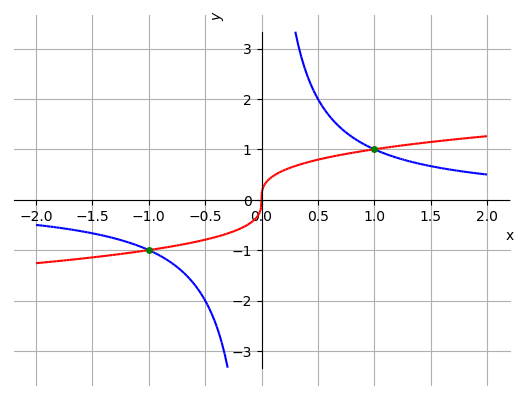
\includegraphics[width=0.6\textwidth]{fig_func/fig_exeresol_funpot_intersep}
    \caption{Interseção dos gráficos das funções $f(x) = 1/x$ (azul) e $g(x) = \sqrt[3]{x}$ (vermelho).}
    \label{fig:exeresol_funpot_intersep}
  \end{figure}

  Agora, basta determinarmos a equação da reta que passa pelos pontos $(x_0, y_0) = (-1, -1)$ e $(x_1, y_1) = (1, 1)$. De \eqref{eq:funafim_eq}, temos que a equação da reta é tal que
  \begin{align*}
    y = \frac{y_1-y_0}{x_1-x_0}(x-x_0)+y_0 &\Rightarrow y = \frac{1-(-1)}{1-(-1)}(x-(-1))+(-1)\\
                                           &\Rightarrow y = x+1-1 \Rightarrow y = x
  \end{align*}
  Ou seja, a que passa pelos pontos de interseção dos gráficos das funções $f(x)$ e $g(x)$ tem equação $y = x$.

  
  Os seguintes comandos, mostrar como podemos resolver este problema usando o GeoGebra:
\begin{verbatim}
A= Interseção(f, g,)
B=Interseção(f, g, 0,6)
x_0=-1
x_1=1
y_0=f(x_0)
y_1=f(x_1)
m=(y_1-y_0)/(x_1-x_0)
y=m(x-x_0)+y_0
\end{verbatim}
\end{resol}
\end{exeresol}

\subsection{Exercícios}\index{Exercícios!função afim}
\begin{exer}
  Faça um esboço do gráfico de cada uma das seguintes funções:
  \begin{multicols}{4}
  \begin{enumerate}[a)]
  \item $f(x) = x$
  \item $g(x) = -x$
  \item $h(x) = x-1$
  \item $t(x) = -x+1$
  \end{enumerate}\end{multicols}
\end{exer}
\begin{resp}
Utilize Applet do GeoGebra disponível \href{https://www.geogebra.org/m/c4mdexgd}{Aqui}.
\end{resp}

\begin{exer}
  Determine a função afim $f(x)=mx+b$, cujo gráfico contém os pontos $(-2, 1)$ e $(0, -2)$.
\end{exer}
\begin{resp}
  $f(x) = -\frac{3}{2}x - 2$
\end{resp}

\begin{exer}
  Dada a função $y = 2x + 3$ determine:
   \begin{opcexer}{a)}
  \item O gráfico
   \item A interseção com o eixo $x$ e com o eixo $y$.
\end{opcexer}
   \end{exer}
\begin{resp}
a) Utilize Applet do GeoGebra disponível \href{https://www.geogebra.org/m/c4mdexgd}{Aqui}.\\
b) $\pc{-\frac{1}{2},0}$ e $(0,3)$
\end{resp}
\begin{exer}
  O custo de um determinado produto é de R\$ 10,00 fixo mais R\$ 2,00 por unidade. Determine:
   \begin{opcexer}{a)}
     \item A equação que expressa o custo em função da  quantidade.
       \item  O gráfico.
         \end{opcexer}
   \end{exer}
\begin{resp}
a) $C(x)=2x+10$\\
b) Utilize Applet do GeoGebra disponível \href{https://www.geogebra.org/m/c4mdexgd}{Aqui}.
\end{resp}
\begin{obs}
 \textit{ Todos os exercícios acima podem ser resolvidos com o auxílio de Applets do GeoGebra disponíveis em \href{https://www.geogebra.org/m/c4mdexgd}{Aqui}.}
\end{obs}

\section{Função quadrática}\label{sec:FuncQuadratica}
\subsection{Definição}\index{Definição!função quadrática}
Os polinômios de grau 2 são, também, chamados de \textbf{funções quadráticas}, i.e. funções da forma
\begin{equation}
  f(x) = ax^2 + bx + c,\label{eq:FormCanFuncQuad}
\end{equation}
onde $a$ é chamado de \textbf{coeficiente do termo quadrático}, $b$ o \textbf{coeficiente do termo linear} e $c$ o \textbf{coeficiente do termo constante}.

\subsection{Raízes ou zeros da função quadrática}\label{subsec:FuncQuad-zeros}
Os zeros de uma função quadrática podem ser calculados pela \textbf{fórmula de Bhaskara}
\begin{equation}\label{eq:Bhaskara}
  x_0, x_1 = \frac{-b \pm \sqrt{b^2 - 4ac}}{2a}
\end{equation}

No ensino médio costuma-se dividir esta fórmula em duas da seguinte maneira:
%\sistemaeq[eq:FormBaskDiv]{\Delta =b^2-4ac}{x=\frac{-b\pm\sqrt{\Delta}}{2a}}
\begin{equation}
\left\{\begin{array}{l} 
\Delta =b^2-4ac\\ x=\frac{-b\pm\sqrt{\Delta}}{2a}\end{array}\right.\label{eq:FormBaskDiv}
\end{equation}
Posteriormente, encontra-se as raízes fazendo 
\begin{equation}
   x_0=\frac{-b+\sqrt{\Delta}}{2a}\qquad x_1=\frac{-b-\sqrt{\Delta}}{2a}\label{eq:x1x2} 
\end{equation}

\begin{obs}
  Costuma-se também utilizar  no lugar de $x_0$ e $x_1$, $x'$ e $x''$, respectivamente.
\end{obs}
Quanto ao número de raízes, uma função quadrática pode admitir duas raízes reais distintas, duas raízes reais iguais (uma única raiz real) ou nenhuma raiz real, a depender do \textbf{discriminante $\Delta$}\index{discriminante}:
\begin{compactenum}[(i)]
\item Se $\boldsymbol{\Delta>0}$, então as raízes $x_0$ e $x_1$ dados pelas fórmulas \ref{eq:x1x2} são distintas, ou seja, \textbf{a função quadrática admite duas raízes reais distintas};
\item Se $\boldsymbol{\Delta=0}$ temos $\sqrt{\Delta}=\sqrt{0}=0$, então  $x_0=x_1=-b/2a$, ou seja, \textbf{a função quadrática admite duas raízes reais iguais (uma única raiz real)};
\item Se $\boldsymbol{\Delta<0}$, então $\sqrt{\Delta}$ não é um número real (é um número complexo), portanto $x_0$ e $x_1$ não são números reais. Em outras palavras, a função não admite raízes reais.
\end{compactenum}
\begin{obs}
 \textbf{ O gráfico da função intercepta o eixo das abscissas  nos valores das raízes}. Portanto, se $\Delta>0$ o gráfico intercepta o eixo das abscissas  em dois pontos, a saber: $(x_0,0)$ e $(x_1,0)$. Se $\Delta=0$ o gráfico intercepta o eixo das abscissas em apenas um ponto. No entanto, se $\Delta<0$ o gráfico da função não intercepta o eixo das abscissas\index{abscissas}.
\end{obs}
Observando os gráficos da Figura  \ref{fig:FuncQuadConcav} podemos deduzir que as raízes são $-1$ e $2$, pois o gráfico intercepta o eixo das abscissas nos pontos $(-1,0)$ e $(2,0)$.\\ \dica Comprove através da fórmula de Bhaskara.
\subsection{Deduzindo a fórmula de Bháskara}\index{Fórmula!Bháskara}\label{subsec:FuncQuad-FormBhaskara}

Sabemos que para encontrar os zeros ou raízes de uma função devemos igualar sua imagem a zero, ou seja, $f(x)=0$. Considerando a equação \ref{eq:FormCanFuncQuad}, temos:
\begin{equation*}
\begin{aligned}
    ax^2+bx+c=0\\
    x^2+\frac{b}{a}x+\frac{c}{a}=0\\
    x^2+\frac{b}{a}x=-\frac{c}{a}\\
    x^2+\frac{b}{a}x+\red{\frac{b^2}{4a^2}}=-\frac{c}{a}+\red{\frac{b^2}{4a^2}}\\
    \pc{x+\frac{b}{2a}}^2=\frac{b^2-4ac}{4a^2}\\
    \pc{x+\frac{b}{2a}}=\pm\sqrt{\frac{b^2-4ac}{4a^2}}\\
      x=-\frac{b}{2a}\pm\frac{\sqrt{b^2-4ac}}{2a}\\
  x=\frac{-b\pm \sqrt{b^2-4ac}}{2a}
\end{aligned}
\end{equation*}
Assim, chegamos a fórmula \ref{eq:x1x2}.
\subsection{Soma e Produto de raízes}\label{subsec:FuncQuad-Soma&Produto}
Dadas as raízes $  x_0=\frac{-b+\sqrt{\Delta}}{2a}\qquad \textrm{ e } x_1=\frac{-b-\sqrt{\Delta}}{2a}$ e o discriminante $\Delta=b^2-4ac$ temos:
\begin{compactenum}[(i)]
\item \textbf{Soma de raízes:}\index{Raízes!soma} $$x_0+x_1=\pc{\frac{-b+\sqrt{\Delta}}{2a}}+\pc{\frac{-b-\sqrt{\Delta}}{2a}}=\frac{-2b}{2a}=\frac{-b}{a}$$
Portanto, 
\begin{equation}
    x_0+x_1=\frac{-b}{a}\label{SomRaizes}
\end{equation}
\item \textbf{Produto de raízes:}\index{Raizes!produto}
\begin{align*}
    x_0\cdot x_1&=\pc{\frac{-b+\sqrt{\Delta}}{2a}}\cdot\pc{\frac{-b-\sqrt{\Delta}}{2a}}\\
   & =\frac{b^2-(\sqrt{\Delta})^2}{4a^2}\\
   &=\frac{b^2-\Delta}{4a^2}=\frac{b^2-(\red{b^2-4ac})}{4a^2}\\
   &=\frac{4ac}{4a^2}=\frac{c}{a}
\end{align*}
Desta forma 
\begin{equation}
    x_0\cdot x_1=\frac{c}{a}\label{ProdRaizes}
\end{equation}
\end{compactenum}
\desafio{Considerando as Fórmulas \ref{SomRaizes} e \ref{ProdRaizes} de soma e produto de raízes de uma função quadrática, deduza o ``macete''~ de como encontrar zeros de uma função quadrática, sem utilizar a fórmula de Bhaskara. }
\subsection{Concavidade}\index{Parábola!concavidade}\label{subsec:FuncQuad-Concavidade}
O esboço do gráfico de uma função quadrática é uma \textbf{parábola côncava para cima}\index{Concavidade!para cima} quando $a > 0$ ou, \textbf{côncava para baixo}\index{Concavidade!para baixo} quando $a < 0$. Veja a Figura \ref{fig:FuncQuadConcav}.
\begin{figure}[H]
  \centering
  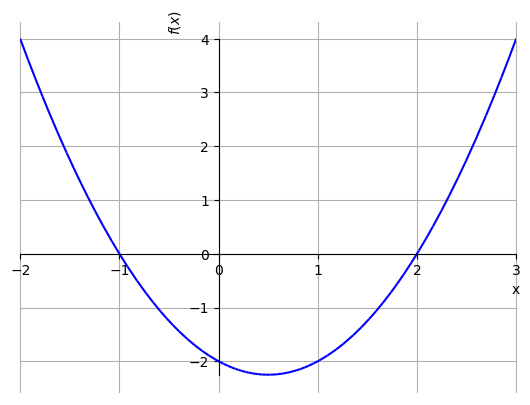
\includegraphics[width=0.5\textwidth]{fig_func/fig_funquad_concavidade_cima}~
    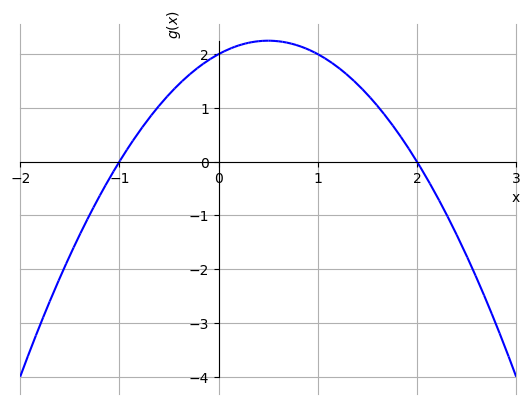
\includegraphics[width=0.5\textwidth]{fig_func/fig_funquad_concavidade_baixo}
  \caption{Esboço dos gráficos das funções quadráticas $f(x) = x^2-x-2$ (esquerda) e $g(x)=-x^2+x+2$ (direita).}
  \label{fig:FuncQuadConcav}
\end{figure}
\subsection{Vértice}\label{subsec:FuncQuad-Vertice}
O \textbf{vértice}\index{Parábola!vértice} da função quadrática $f(x)$ é o ponto de coordenadas $x_v$ e $y_v$, indicado por $\boldsymbol{(x_v,y_v)}$, no qual a função admite valor mínimo (quando $a>0$) ou valor máximo (quando $a<0$). 

Quando $f$ têm zeros reais, o ponto de abscissa do vértice é o ponto médio entre os zeros $x_0$ e $x_1$ da função, i.e. o vértice $V = (x_v, y_v)$ é tal que
\begin{equation}
  x_v = \frac{x_0 + x_1}{2},\quad\text{e}\quad y_v = f(x_v). 
\end{equation}
O valor $x_v$ é a abscissa do ponto em que a função quadrática $f$ atinge o valor máximo (valor mínimo) $y_v$.

Executando a operação matemática $x_v = \frac{x_0 + x_1}{2}$ com as expressões de $x_0$ e $x_1$ em \ref{eq:x1x2}, chegamos a 
\begin{equation}
    x_v=\frac{-b}{2a}\label{eq:FormXv}
\end{equation}
(\dica Experimente a comprovação).

Substituindo  $x_v$ da equação \ref{eq:FormXv} na expressão \ref{eq:FormCanFuncQuad} e levando em consideração \ref{eq:FormBaskDiv},  encontramos 
\begin{equation}
    y_v=\frac{-\Delta}{4a}\label{eq:FormYv}
\end{equation}

Segue que das Fórmulas \ref{eq:FormXv} e \ref{eq:FormYv} podemos escrever a fórmula do vértice da parábola como 
\begin{equation}
    V = \left(\frac{-b}{2a}, \frac{-\Delta}{4a}\right)\label{eq:VertParab}
\end{equation}

Portanto, quando a parábola está voltada para cima a função admite valor mínimo e quando está voltada para baixo a função admite valor mínimo. Em ambos os casos o valor mínimo ou máximo é  $y_v=-\Delta/4a$, para $x_v=-b/2a$ e o vértice é indicado pela Fórmula \ref{eq:VertParab}.

No caso da Figura \ref{fig:FuncQuadConcav}, no gráfico da esquerda, temos uma parábola voltada para cima, portanto a função admite valor mínimo igual a $y_v=-9/4$ para $x=1/2$. Já no gráfico da direita, a parábola está voltada para baixo, neste caso a função admite valor máximo igual a $y_v=-9/4$ para $x=1/2$ (Cálculos no Exercício Resolvido \ref{Exer:ExercConcav}) e, portanto, o vértice é dado por
\matt{
V=\pc{\frac{1}{2},\frac{9}{4}}
}

A Figura \ref{fig:ResumoFuncQuad} resume o que foi discutido sobre concavidade, número de raízes e vértice da função quadrática, da seguinte forma:
\begin{compactenum}[(i)]
\item $\boldsymbol{a>0$ e $\Delta <0}$ - A função tem concavidade voltada para cima, tem um valor mínimo dado pela Equação \ref{eq:FormYv}. Além disso não admite raízes reais e, portanto seu gráfico não intercepta o eixo das abscissas;
\item $\boldsymbol{a>0$ e $\Delta =0}$ - A função tem concavidade voltada para cima, tem um valor mínimo dado pela Equação \ref{eq:FormYv} que corresponde a $0$, pois $\Delta=0$. Admite apenas uma raiz real  $x=-b/2a$  e seu gráfico  intercepta o eixo das abscissas em apenas um ponto.
\item $\boldsymbol{a>0$ e $\Delta >0}$ - A função tem concavidade voltada para cima, tem um valor mínimo dado pela Equação \ref{eq:FormYv}. Admite duas raízes reais distintas e, portanto, seu gráfico  intercepta o eixo das abscissas em dois pontos distintos.
\item $\boldsymbol{a<0$ e $\Delta <0}$ - A função tem concavidade voltada para baixo, tem um valor máximo dado pela Equação \ref{eq:FormYv}. Além disso não admite raízes reais e, portanto seu gráfico não intercepta o eixo das abscissas;
\item $\boldsymbol{a<0$ e $\Delta =0}$ - A função tem concavidade voltada para baixo, tem um valor máximo dado pela Equação \ref{eq:FormYv} que corresponde a $0$, pois $\Delta=0$. Admite apenas uma raiz real dada por $x=-b/2a$  e seu gráfico  intercepta o eixo das abscissas em apenas um ponto
\item $\boldsymbol{a<0$ e $\Delta >0}$ - A função tem concavidade voltada para baixo, tem um valor máximo dado pela Equação \ref{eq:FormYv}. Admite duas raízes reais distintas e, portanto, seu gráfico  intercepta o eixo das abscissas em dois pontos distintos.
\end{compactenum}
\begin{figure}[H]
  \centering
  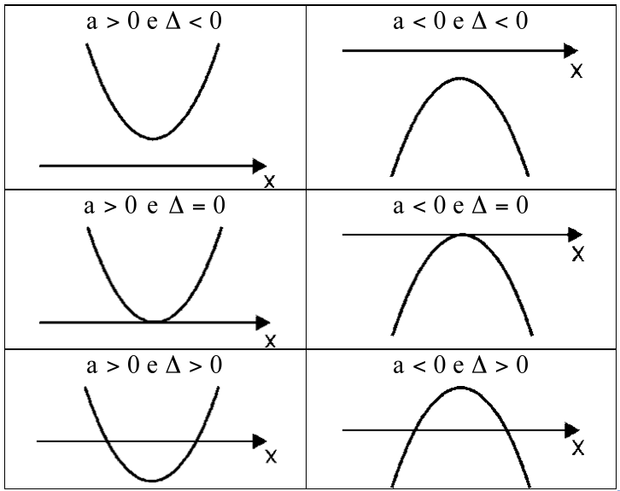
\includegraphics[width=0.8\textwidth]{fig_func/ParabValorDeltaA}
  \caption{Resumo da concavidade e número de raízes da função quadrática.}
  \label{fig:ResumoFuncQuad}
\end{figure}
\subsection{Exercícios resolvidos}
\begin{exeresol}
  Determine os zeros do polinômio $f(x) = x^3-x^2-2x$.
  \begin{resol}
  Determinar os zeros da função $f$ significa entrar todos os valores de $x$ tais que $f(x)=0$ (estes são as abscissas dos pontos nos quais o gráfico de $f$ intersepta o eixo das abscissas). Temos
  \begin{align*}
    f(x)=0 &\Rightarrow x^3-x^2-2x=0 \Rightarrow x(x^2-x-2)=0\\
           &\Rightarrow x=0\quad\text{ou}\quad x^2-x-2=0
  \end{align*}
  Então, usando a fórmula de Bhaskara \eqref{eq:Bhaskara} na equação $x^2-x-2=0$, obtemos
  \begin{align*}
    x &= \frac{-b\pm\sqrt{b^2-4ac}}{2a} \\
      &= \frac{1\pm\sqrt{1-4\cdot 1\cdot (-2)}}{2}\\
      &= \frac{1\pm\sqrt{9}}{2}= \frac{1\pm 3}{2}\\
      &= -1\quad\text{ou}\quad 2
  \end{align*}
  Com isso, temos que os zeros da função $f$ ocorrem nos pontos $x_0 = -1$, $x_1=0$ e $x_2=2$.

  
  Com o \geogebra, podemos calcular os zeros da função $f$ com os seguintes comandos:
\begin{verbatim}
f(x)=x^2-x-2
raiz(f)
\end{verbatim}
\end{resol}
\end{exeresol}
\begin{exeresol}\label{Exer:ExercConcav}
  Determine o valor mínimo da função $f(x) = x^2 - x - 2$.
  \begin{resol}
  Como $f$ é uma função quadrática com coeficiente quadrático positivo, temos que seu gráfico é uma parábola côncava para cima. Logo, $f$ atinge seu valor mínimo no seu vértice. Por sorte, os zeros de $f$ são $x_0 = -1$ e $x_1 = 2$. Logo, o vértice tem abscissa
  \begin{equation*}
    x = \frac{x_0 + x_1}{2} = \frac{1}{2}
  \end{equation*}
  Ou seja, a abscissa do ponto de mínimo de $f$ é $1/2$ e seu valor mínimo é
  \begin{equation*}
    f\left(\frac{1}{2}\right) = \left(\frac{1}{2}\right)^2-\frac{1}{2}-2 = \frac{1-2-8}{4} = -\frac{9}{4}
  \end{equation*}
\begin{obs}
  Poderíamos ter resolvido este exercício utilizando as fórmulas de $x_v$ (\ref{eq:FormXv}) e  $y_v$ (\ref{eq:FormYv}).
\end{obs}
  Podemos resolver este exercício com o seguinte código \geogebra:
\begin{verbatim}
f(x)=x^2 - x - 2
t=Soluções(f)
f((t(1) + t(2)) / 2)
\end{verbatim}

O \geogebra~ também fornece direto o vértice através do comando \verb+Extremo+
\begin{verbatim}
f(x)=x^2 - x - 2
Extremo(f)
\end{verbatim}
\end{resol}
\end{exeresol}

\begin{minipage}{0.68\linewidth}
\begin{exeresol}
 Uma pessoa quer construir um galinheiro de forma retangular,
 usando um muro reto já construído como um dos lados do galinheiro.
 Dado que essa pessoa tem material para construir 60 metros de cerca de 
uma altura fixa,  determine os valores de $x$ e $z$,  de modo que a área do galinheiro seja a maior possível (possa abrigar o maior número possível de galinhas).\\
A figura ao lado ilustra o problema.
\end{exeresol}
\end{minipage}\hfill
\begin{minipage}{0.26\linewidth}
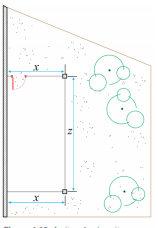
\includegraphics[scale=0.8]{1-cap_func/fig_func/Galinheiro}
\end{minipage}


\begin{resol}
     Tendo em vista que o galinheiro é retangular,  a sua área,  denominada $y$, é dada pelo produto dos lados:
  \matt{
  y=xz
  }
  
  Os lados $x$ e $z$ devem respeitar a limitação imposta pela quantidade 
de material à disposição.
 Assim, escrevemos para a soma dos três lados do galinheiro:
 \matt{x+z+x=60}
  
  Donde concluímos que,  com o material existente,
 a relação entre os lados é dada por:
 \matt{z=60-2x}
 
  Portanto,  escrevendo a área da construção em função do comprimento do lado,  $x$, obtemos:
 \matt{
 y=x(60-2x)=2x^2+60x
 }
 
Como $a < 0$,  a concavidade da parábola,  que é o gráfico da função $y = f( x )$, 
 é para baixo e a função admite um valor máximo para a abscissa dada por:
 $$x=x_v=\frac{-b}{a}=\frac{-60}{2\cdot(-2)}=15$$
Assim,  para esse valor de x,  o valor do outro lado será dado por:
\matt{z=60-2x=60-2\cdot 15=30}
Portanto,  para que o galinheiro tenha a área máxima,  devemos ter:\\
\begin{center} $x=15\; metros$ e $z=30\; metros$\end{center}
\end{resol} 
\subsection{Exercícios}
\begin{exer}
  Determine as raízes, o vértice e o gráfico das seguintes funções:
  \begin{multicols}{3}
  \begin{compactenum}[a)]
  \item $x^2-6x+8$ \item $-x^2+4x-4$\item $2x^2+4x+5$
  \end{compactenum}
 \end{multicols}
\end{exer}
\begin{resp}
\begin{multicols}{2}
  \begin{compactenum}[a)]
  \item Raízes: 2 e 4, vértice: $(3,-1)$ \item Raiz: 2 , vértice: $(2,0)$\item não tem raízes reais, vértice: $(-1,3)$
  \end{compactenum}
 \end{multicols}
\end{resp}
\begin{exer}
  A trajetória da bola, num chute a gol, descreve uma parábola. Supondo que sua altura $h$, em metros, $t$ segundos após o chute, seja dada por  $h = -t^2 + 6 t$, determine a altura máxima atingida pela bola.
\end{exer}
\begin{resp}
$9$ metros
\end{resp}
\begin{exer}
   Uma parede de tijolos será usada como um dos lados de um curral retangular. Para os outros lados, iremos usar 400 metros de tela de arame, de modo a produzir uma área máxima.\\
Então o quociente de um lado pelo outro é
\begin{multicols}{5}
\begin{compactenum}[a)]
\item  1\item  0,5\item  2,5\item  3\item 1,5
\end{compactenum}
\end{multicols}
\end{exer}
\begin{resp}
  b
\end{resp}
\begin{obs}
 \textit{ Todos os exercícios acima podem ser resolvidos com o auxílio de Applets do GeoGebra disponíveis em \href{https://www.geogebra.org/m/pnscwa4e}{Aqui}.}
\end{obs}

\section{Funções trigonométricas}\label{sec:FuncTrigonometricas}
\subsection{Seno e cosseno}\index{Trigonometria!seno e cosseno}\label{subsec:Trig_Seno-cosseno}
As funções trigonométricas\index{Função!trigonométricas} seno \boldmat{$y=\sen(x)$} e cosseno $\boldsymbol{y=\cos(x)}$ podem ser definidas a partir do círculo trigonométrico (veja a Figura \ref{fig:cos_seno}). Seja $x$ o ângulo\footnote{Em geral utilizaremos a medida em radianos para ângulos.} de declividade da reta que passa pela origem do plano cartesiano (reta $r$ na Fig. \ref{fig:cos_seno}). 
\begin{figure}[H]
  \centering
  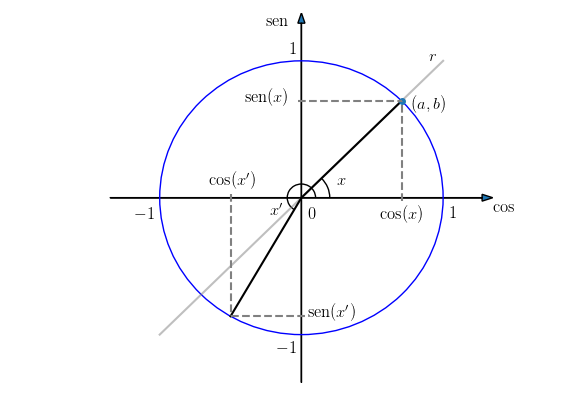
\includegraphics[width=0.8\textwidth]{fig_func/fig_cos_seno}
    \caption{Funções seno e cosseno no círculo trigonométrico.}
  \label{fig:cos_seno}
\end{figure}
Seja, então, $(a,b)$ o ponto de interseção desta reta com a circunferência unitária\footnote{Circunferência do círculo de raio 1.}. Então, definimos:
\begin{equation}
  \cos(x) = a,\qquad \sen(x) = b.
\end{equation}
A partir da definição, notemos que ambas funções têm domínio $(-\infty, \infty)$ e imagem $[-1, 1]$.

Na Figura \ref{fig:cos_seno_valores} podemos extrair os valores das funções seno e cosseno para os ângulos fundamentais. Por exemplo, temos
\begin{align*}
  &\sen\left(\frac{\pi}{6}\right) = \frac{1}{2}\qquad\qquad\quad \cos\left(\frac{\pi}{6}\right) = \frac{\sqrt{3}}{2}\\
  &\sen\left(\frac{3\pi}{4}\right) = \frac{\sqrt{2}}{2}\qquad\qquad \cos\left(\frac{\pi}{4}\right) = -\frac{\sqrt{2}}{2}\\
  &\sen\left(\frac{8\pi}{6}\right) = -\frac{\sqrt{3}}{2}\qquad\quad \cos\left(\frac{8\pi}{6}\right) = -\frac{1}{2}\\
  &\sen\left(\frac{11\pi}{6}\right) = -\frac{1}{2}\qquad\qquad \cos\left(\frac{11\pi}{6}\right) = \frac{\sqrt{3}}{2}\\
\end{align*}
\begin{figure}[H]
  \centering
  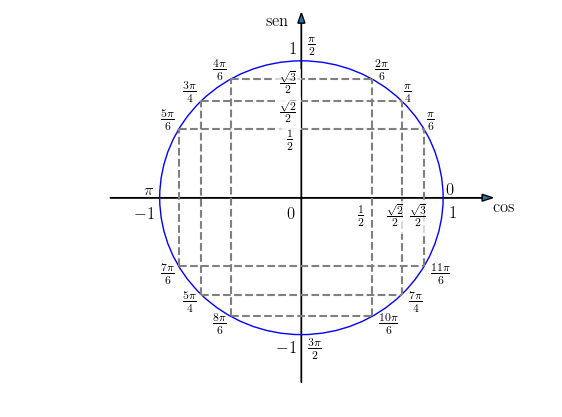
\includegraphics[width=0.8\textwidth]{fig_func/fig_cos_seno_valores}
  \caption{Funções seno e cosseno no círculo trigonométrico.}
  \label{fig:cos_seno_valores}
\end{figure}
\dica As funções seno e cosseno estão definidas no \geogebra~como \verb+sin+ e $\verb+cos+$, respectivamente. Por exemplo, para computar o seno de $\pi/6$, digitamos: \verb+sin(pi/6)+

Uma {\bf função} $f(x)$ é dita {\bf periódica}\index{Função!!periódica} quando existe um número $p$, chamado de período da função, tal que
\begin{equation}
  f(x+p) = f(x)
\end{equation}
para qualquer valor de $x$ no domínio da função. Da definição das funções seno e cosseno, notemos que ambas são periódicas com período $2\pi$, i.e.
\begin{equation}
  \sen(x+2\pi) = \sen(x),\qquad \cos(x+2\pi) = \cos(x),
\end{equation}
para qualquer valor de $x$.

Na Figura \ref{fig:cos_seno_graficos}, temos os esboços dos gráficos das funções seno e cosseno.

\begin{figure}[H]
  \centering
  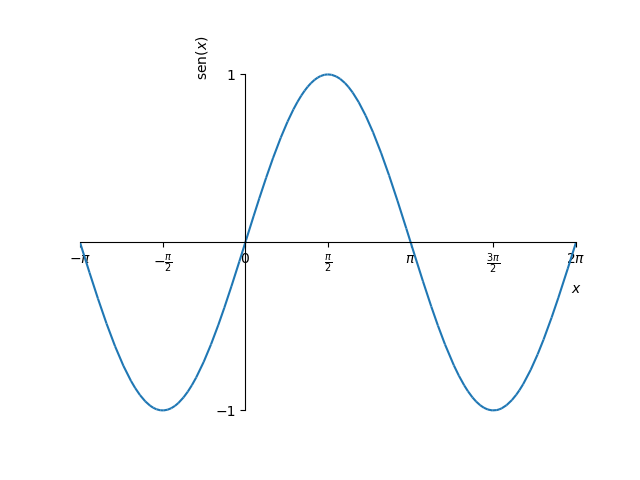
\includegraphics[width=0.5\textwidth]{fig_func/fig_seno_grafico}~
  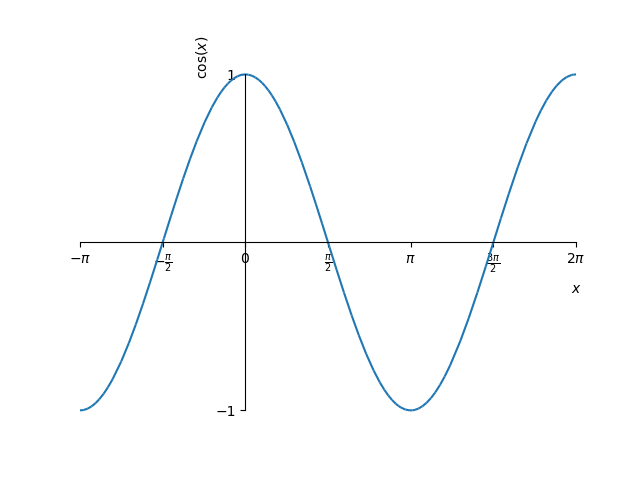
\includegraphics[width=0.5\textwidth]{fig_func/fig_cosseno_grafico}
  \caption{Esboços dos gráficos das funções seno (esquerda) e cosseno (direita).}
  \label{fig:cos_seno_graficos}
\end{figure}
\subsection{Tangente, cotangente, secante e cossecante}\label{subsec:Tang-Cot-Sec-Cossecante}
Das funções seno e cosseno, definimos as funções {\bf tangente}\index{Função!!tangente}, {\bf cotangente}\index{Função!!cotangente}, {\bf secante}\index{Função!!secante} e {\bf cossecante}\index{Função!!cossecante} como seguem:
\begin{align*}
  \tg(x) = \frac{\sen(x)}{\cos(x)}\qquad\qquad \cotg(x) = \frac{\cos(x)}{\sen(x)}\\
  \sec(x) = \frac{1}{\cos(x)}\qquad\qquad \cosec(x) = \frac{1}{\sen(x)}
\end{align*}

\dica No \geogebra, as funções tangente, cotangente, secante e cossecante podem ser computadas com as funções $\verb+tan+$, $\verb+cot+$, $\verb+sec+$ e $\verb+csc+$, respectivamente. Por exemplo, podemos computar o valor de $\cosec(\pi/4)$ com o comando: \verb+csc(pi/4)+

Na Figura \ref{fig:co_tg_graficos}, temos os esboços dos gráficos das funções tangente e cotangente. Observemos que a função tangente não está definida nos pontos $(2k+1)\pi/2$, para todo $k$ inteiro. Já, a função cotangente não está definida nos pontos $k\pi$, para todo $k$ inteiro. Ambas estas funções têm imagem $(-\infty, \infty)$ e período $\pi$.

\begin{figure}[H]
  \centering
  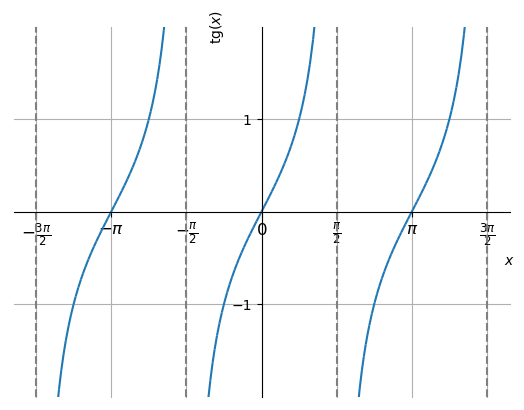
\includegraphics[width=0.5\textwidth]{fig_func/fig_tg_grafico}~
  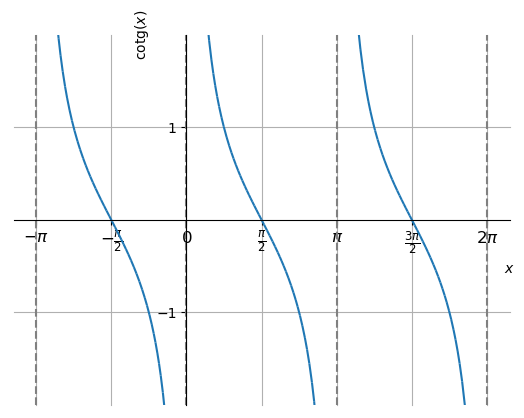
\includegraphics[width=0.5\textwidth]{fig_func/fig_cotg_grafico}
  \caption{Esboços dos gráficos das funções tangente (esquerda) e cotangente(direita).}
  \label{fig:co_tg_graficos}
\end{figure}

Na Figura \ref{fig:co_sec_graficos}, temos os esboços dos gráficos das funções secante e cossecante. Observemos que a função secante não está definida nos pontos $(2k+1)\pi/2$, para todo $k$ inteiro. Já, a função cossecante não está definida nos pontos $k\pi$, para todo $k$ inteiro. Ambas estas funções têm imagem $(-\infty, 1]\cup [1, \infty)$ e período $\pi$.

\begin{figure}[H]
  \centering
  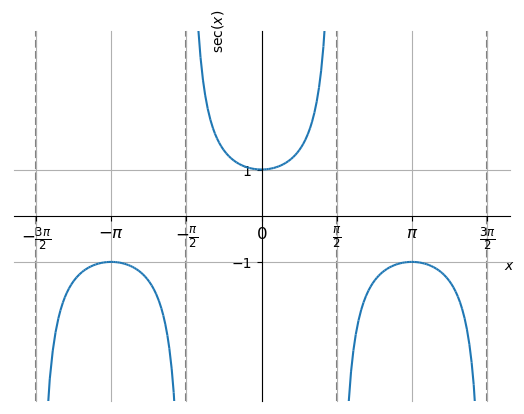
\includegraphics[width=0.5\textwidth]{fig_func/fig_sec_grafico}~
  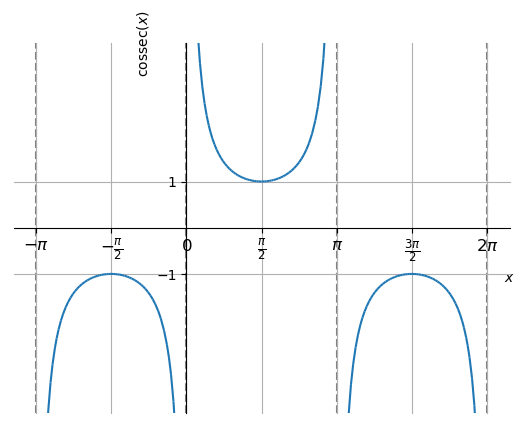
\includegraphics[width=0.5\textwidth]{fig_func/fig_cosec_grafico}
  \caption{Esboços dos gráficos das funções secante (esquerda) e cossecante (direita).}
  \label{fig:co_sec_graficos}
\end{figure}
\subsection{Identidades trigonométricas}\label{subsec:IdentTrigometricas}
Aqui, vamos apresentar algumas identidades trigonométricas\index{Trigonometria!identidades} que serão utilizadas ao longo do curso de cálculo. Comecemos pela identidade fundamental
\begin{equation}
  \sin\!\!^2 x + \cos^2 x = 1\label{eq:IdentTrig}
\end{equation}
Desta decorrem as identidades
\begin{align}
  &\tg\!\!^2(x) + 1 = \sec^2 x\label{eq:tan^2}\\
  &1 + \cotg^2(x) = \cosec^2(x)\label{eq:cotan^2}
\end{align}

Das seguintes fórmulas para adição/subtração de ângulos
\begin{align}
  &\cos(x\pm y) = \cos(x)\cos(y) \mp \sen(x)\sen(y)\label{eq:CosSomDif}\\
  &\sen(x\pm y) = \sen(x)cos(y) \pm \cos(x)\sen(y)\label{eq:SenSomDif}
\end{align}
seguem as fórmulas para ângulo duplo
\begin{align}
  &\cos(2x) = \cos^2x - \sen\!\!^2x\\
  &\sen(2x) = 2\sen x\cos x
\end{align}

Também, temos as fórmulas para o ângulo metade
\begin{align}
  &\cos^2 x = \frac{1 + \cos 2x}{2}\label{eq:CosDuplo}\\
  &\sen\!\!^2 x = \frac{1 - \cos 2x}{2}\label{eq:SenDuplo}
\end{align}
\subsection{Exercícios resolvidos}\index{Exercícios resolvidos!func. trigonométricas}
\begin{exeresol}
  Mostre que
  \begin{equation*}
    \cos x - 1 = -2\sen\!\!^2 \frac{x}{2}
  \end{equation*}
  \begin{resol}
  A identidade trigonométrica
  \begin{equation*}
    \sen\!\!^2 x = \frac{1 - \cos 2x}{2},
  \end{equation*}
  aplicada a metade do ângulo, fornece
  \begin{equation*}
    \sen\!\!^2 \frac{x}{2} = \frac{1 - \cos x}{2}
  \end{equation*}
  Então, isolando $\cos x$, obtemos
  \begin{align*}
    \sen\!\!^2 \frac{x}{2} = \frac{1 - \cos x}{2} &\Rightarrow 1 - \cos x = 2\sen\!\!^2 \frac{x}{2}\\
                                              &\Rightarrow \cos x - 1 = -2\sen\!\!^2 \frac{x}{2}
  \end{align*}
\end{resol}
\end{exeresol}

\subsection{Exercícios}\index{Exercícios!func. trigonométricas}
\begin{exer}
  Demonstre a identidade trigonométrica\index{Trigonometria!identidades} \ref{eq:IdentTrig}.
\end{exer}
\begin{resp}
  Dica: Utilize o Teorema de Pitágoras.
\end{resp}

\begin{exer}
  Demonstre as Fórmulas \ref{eq:tan^2} e \ref{eq:cotan^2}, utilizando a identidade \ref{eq:IdentTrig}.
  \end{exer}
\begin{resp}
\end{resp}

\begin{exer}
  Demonstre as Fórmulas \ref{eq:CosDuplo} e \ref{eq:SenDuplo} com base nas Fórmulas \ref{eq:CosSomDif} e \ref{eq:SenSomDif}.
\end{exer}
\section{Operações com funções}\index{Função!operações}\label{subsec:Func-Operacoes}
\subsection{Somas, diferenças, produtos e quocientes}
Sejam dadas as funções $f$ e $g$ com domínio em comum $D$. Então, definimos as funções
\begin{itemize}
\item $(f\pm g)(x) = f(x) \pm g(x)$ para todo $x\in D$;
\item $(fg)(x) = f(x)g(x)$ para todo $x\in D$;
\item $\displaystyle \left(\frac{f}{g}\right)(x) = \frac{f(x)}{g(x)}$ para todo $x\in D$ tal que $g(x)\neq 0$.
\end{itemize}

\begin{ex}
  Sejam $f(x)=x^2$ e $g(x)=x$. Temos:
  \begin{itemize}
  \item $(f+g)(x) = x^2 + x$ e está definida em toda parte.
  \item $(g-f)(x) = x - x^2$ e está definida em toda parte.
  \item $(fg)(x) = x^3$ e está definida em toda parte.
  \item $\left(\frac{f}{g}\right)(x) = \frac{x^2}{x}$ e tem domínio $(-\infty, \infty)\setminus \{0\}$\footnote{Observemos que não podemos simplificar o $x$, pois a função $y=x$ é diferente da função $y=x^2/x$.}.
  \end{itemize}
\end{ex}

\subsection{Composição de funções}\label{subsec:Composicao-Funcoes}
Sejam \(f:A\rightarrow B\) e \(g:B\rightarrow C\) duas funções reais tais que \({\rm Im}(f)\cap {\rm Dom}(g)\not=\emptyset\). A composição de \(g\) com \(f\), denotada por \(g\circ f\), é a função \(g\circ f : A\rightarrow C\) definida por:

\[ (g\circ f)(x)=g(f(x)). \]
O domínio da função composta \(g\circ f\) é dado por

\[ {\rm Dom}(g\circ f) = \left\{ x\in \mathbb{R}\,:\, x\in {\rm Dom}(f) \mbox{ e } f(x)\in{\rm Dom}(g) \right\}. \]
Na Figura \ref{fig:Compfunc}, ilustramos a função composta \(g\circ f\)
\begin{figure}[!htb]
    \centering
    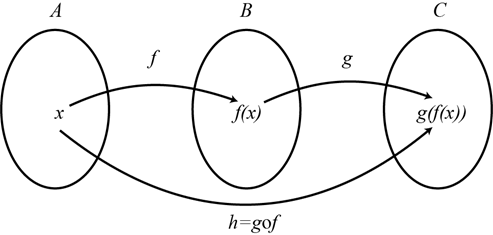
\includegraphics[scale=0.8]{1-cap_func/fig_func/Repres-Funcao-composta.png}
    \caption{Representação da composição de funções}
    \label{fig:Compfunc}
\end{figure}

\nota{
  Em geral,  a operação de composição de funções não é comutativa, isto é,
  $$(f\circ g)(x)\neq (g\circ f)(x)$$

  Uma função composta com sua inversa e vice versa é igual a função identidade, ou seja,
  \matt{
  (f\circ f^{-1})(x)=(f^{-1}\circ f)(x)=x
  }
}
\begin{ex}
  Sejam $f(x) = x^2$ e $g(x) = x+1$. A função composta $f\circ g$ é dada por $(f\circ g)(x) = f(g(x)) = f(x+1) = (x+1)^2$.
\end{ex}

\begin{ex}
Sejam as funções \(f(x)=2x-6\) e \(g(x)=\sqrt{x}\). Encontre o domínio de \(g\circ f\) e \(f\circ g\).\\
\begin{solution}
\((g\circ f)(x)=g(f(x))= g\left(2x-6\right)=\sqrt{2x-6} \),
logo, o domínio da \(g\circ f\) é

\[ \begin{array}{rcl} {\rm Dom}(g\circ f) &=& \left\{ x\in \mathbb{R}\,:\, x\in {\rm Dom}(f) \mbox{ e } f(x)\in{\rm Dom}(g) \right\}\\ &=& \left\{ x\in \mathbb{R}\,:\, x\in \mathbb{R} \mbox{ e } 2x-6\geq 0 \right\}\\ &=& [3,+\infty) \end{array} \]
\((f\circ g)(x)=f(g(x))= f\left(\sqrt{x}\right)=2\sqrt{x}-6\),
logo, o domínio da \(f\circ g\) é
\[ \begin{array}{rcl} {\rm Dom}(f\circ g) &=& \left\{ x\in \mathbb{R}\,:\, x\in {\rm Dom}(g) \mbox{ e } g(x)\in{\rm Dom}(f) \right\}\\ &=& \left\{ x\in \mathbb{R}\,:\, x\geq 0 \mbox{ e } \sqrt{x}\in \mathbb{R} \right\}\\ &=& [0,+\infty) \end{array} \]
\end{solution}
\end{ex}
\subsection{Função Inversa}\index{Função!inversa}\label{subsec:FuncInversa}
Dada uma função \(f: A\rightarrow B\), gostaríamos de saber como o efeito de uma função pode ser invertido para enviar o resultado de volta e obter o valor de onde veio. Nossa resposta seria: se \(f(x)=y\), então \(x=f^{-1}(y)\), mas não necessariamente sempre obtemos uma função.

De fato, sempre temos alguma das duas possibilidades: \(f\) é injetora ou \(f\) não é injetora.
\begin{itemize}
    \item Se \(f\) não é injetora, existem pelo menos dois elementos \(x_1,x_2\in A\) tais que:

\[f(x_1)=y \quad \mbox{e} \quad f(x_2)=y\quad \mbox{então}\quad x_1=f^{-1}(y) \quad \mbox{e} \quad x_2=f^{-1}(y). \]
Portanto, a (relação) inversa de \(f\), \(f^{-1}\), não é uma função de \(B\) em \(A\).

\item Se \(f: A\rightarrow B\) é injetora, então a inversa \( f^{-1}: B\rightarrow A\) é uma função injetora e é chamada de função inversa de \(f\).
\end{itemize}

Em outras palavras, podemos dizer que uma função $y=f(x)$ é dita invertível, ou admite inversa, se existe uma única função $g$ tal que
\begin{equation*}
  g(f(x)) = x,
\end{equation*}
para todo $x$ no domínio da $f$. Tal função $g$ é chamada de {\bf função inversa}\index{Função!!inversa} de $f$ é comumente denotada por $f^{-1}$.\footnote{Observe que, em geral, $f^{-1} \neq \frac{1}{f}$.}
\begin{framed}
\begin{prop}\label{prop:CompFuncInv}
Duas funções \f~\! e \g são inversas uma da outra se, e somente se, \matt{(f\circ g)(x)=(g\circ f)(x)=x}
\end{prop}\end{framed}
\desafio{Com base na proposição \ref{prop:CompFuncInv}, mostre que as funções exponencial e logarítmica, definidas respectivamente por $f(x)=a^x$ e $g(x)=\log_a x$ são inversas uma da outra.}

\subsubsection{Propriedades da função inversa}
Seja \(f\) uma função. Então:
\begin{itemize}
    \item \(f\) tem inversa se, e somente se, \(f\) for injetora; e neste caso:
\begin{itemize}
    \item  \({\rm Dom}(f^{-1})={\rm Im}(f)\);

\item \({\rm Im}(f^{-1})={\rm Dom}(f)\);

\item \((f^{-1}\circ f)(x)=x\), \(\,\,\,\forall\,x\in {\rm Dom}(f)\);

\item \((f\circ f^{-1})(y)=y\), \(\,\,\,\forall\,y\in {\rm Dom}(f^{-1})\);
\end{itemize}
\item os gráficos de \(y=f(x)\) e \(y=f^{-1}(x)\) são simétricos com respeito à reta \(L:\,\,\,y=x\); 
\item Sejam as funções \(f\) e \(g\) injetoras. Se existe \(g\circ f\), então \((g\circ f)^{-1}= f^{-1}\circ g^{-1}\).
\end{itemize}
\nota{
  Seja \(f\) uma função real definida por \(y=f(x)\) a qual tem função inversa \(f^{-1}\). Para encontrar a regra de correspondência da \(f^{-1}\), colocamos \(x\) em evidência em termos da variável \(y\). Assim, obtemos \(x=f^{-1}(y)\); porém a convenção de representar a variável independente por \(x\) e a variável dependente por \(y\), faz com que escrevamos \(f^{-1}\) em função de \(x\), isto é, trocando as variáveis \(x\) e \(y\) em \(x=f^{-1}(y)\), para obter \(y=f^{-1}(x)\).
}
\begin{ex}
Encontremos a função inversa da função \( f(x)=5x-3\), se \(x\in[0,6]\).\\
\begin{solution}
Da definição de \(f\), verificamos que $f(x_1)=f(x_2)\Rightarrow 5x_1-3=5x_2-3 \Rightarrow x_1=x_2$, assim, \(f\) é injetora e admite inversa. Por outro lado, desde que \(y=f(x)\), então \(y=5x-3\), \(x\in [0,6]\). Pondo em evidência a variável \(x\) obtemos que \(x=\dfrac{y+3}{5}\), para \(x\in [0,6]\). Agora, podemos determinar como varia a variável \(y\):

\[ x=\dfrac{y+3}{5}\in [0,6] \Rightarrow 0\leq \dfrac{y+3}{5} \leq 6 \Rightarrow 0\leq y +3 \leq 30 \Rightarrow -3\leq y \leq 27 \Rightarrow y\in[-3,27] \]
Assim, \(x=\dfrac{y+3}{5}\), para \(y\in [-3,27]\), permutamos \(x\) por \(y\), isto é, \(y=\dfrac{x+3}{5}\), para \(x\in [-3,27]\). Portanto, \(f^{-1}(x)=\dfrac{x+3}{5}\), para \(x\in [-3,27]\).
\end{solution}
\end{ex}
\begin{ex}
Calcule  a função inversa de $f(x) = x^3 + 1$.\\ 
\begin{solution}
Para tando, escrevemos
  \begin{equation*}
    y = x^3 + 1
  \end{equation*}
  Então, isolando $x$, temos
  \begin{equation*}
    x = \sqrt[3]{y - 1}
  \end{equation*}
  Desta forma, concluímos que $f^{-1}(x) = \sqrt[3]{x-1}$. Verifique que $f^{-1}(f(x)) = x$ para todo $x$ no domínio de $f$.
\end{solution}
\end{ex}
\nota{
 Os gráficos de uma dada função injetora $f$ e de sua inversa $f^{-1}$ são simétricos em relação a {\bf reta identidade}\index{reta!identidade} $y=x$.
}
\subsubsection{Exercícios}\index{Exercícios!func.inversa}
\begin{exer}
  Encontre a inversa da função $f(x)=\frac{x}{2}-4$ e mostre que a composição de \f~\!com sua inversa resulta na função identidade
\end{exer}
\subsection{Translações, contrações, dilatações e reflexões de gráficos}\label{subsec:Trans-dilat-cont-reflexao}
Algumas operações com funções produzem resultados bastante característicos no gráfico de funções. Com isso, podemos usar estas operações para construir gráficos de funções mais complicadas a partir de funções básicas.
\subsection{Translações}\index{Função!translação}
Dada uma função $f$ e uma constante $k\neq 0$, temos que a o gráfico de $y = f(x) + k$ é uma translação vertical do gráfico de $f$. Se $k>0$, observamos uma translação vertical para cima. Se $k<0$, observamos uma translação vertical para baixo.\\

\begin{ex}
  Seja $f(x) = x^2$. A Figura \ref{fig:ex_trans_vert}, contém os esboços dos gráficos de $f(x)$ e $f(x)+k = x^2+k$ para $k=1$.

  \begin{figure}[H]
    \centering
    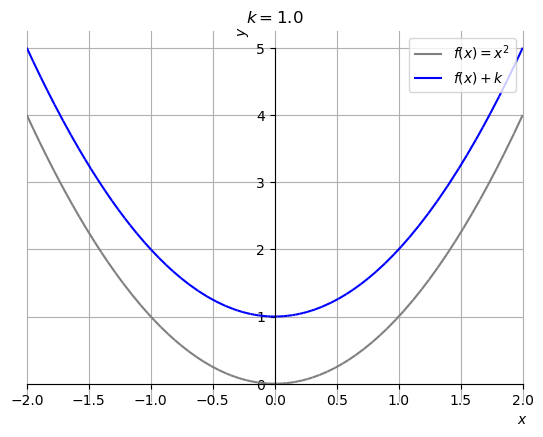
\includegraphics[width=0.6\textwidth]{fig_func/fig_ex_transvert}
    \caption{Esboço do gráfico de $f(x) = x^2$ e $f(x)+k$ com $k=1$.}
    \label{fig:ex_trans_vert}
  \end{figure}

  
 No GeoGebra é possível fazer esboço dos gráficos de $f(x)$ e $f(x)+k$ da seguinte maneira:
\begin{verbatim}
k = 1
f(x)=x^2
f(x)+k
\end{verbatim}
  Observe que o valor de $k$ no \geogebra~ aparece como controle deslizante que pode ser alterado a vontade, permitindo vermos o efeito das translações verticais (\dica Experimente!).
\end{ex}

\vspace{0.3cm}
Translações horizontais de gráficos podem ser produzidas pela soma de uma constante não nula ao argumento da função. Mais precisamente, dada uma função $f$ e uma constante $k\neq 0$, temos que o gráfico de $y=f(x+k)$ é uma translação horizontal do gráfico de $f$ em $k$ unidades. Se $k>0$, observamos uma translação horizontal para a esquerda. Se $k<0$, observamos uma translação horizontal para a direita.\\

\begin{ex}
  Seja $f(x) = x^2$. A Figura \ref{fig:ex_transhoriz}, contém os esboços dos gráficos de $f(x)$ e $f(x+k) = (x+k)^2$ para $k=1$.

  \begin{figure}[H]
    \centering
    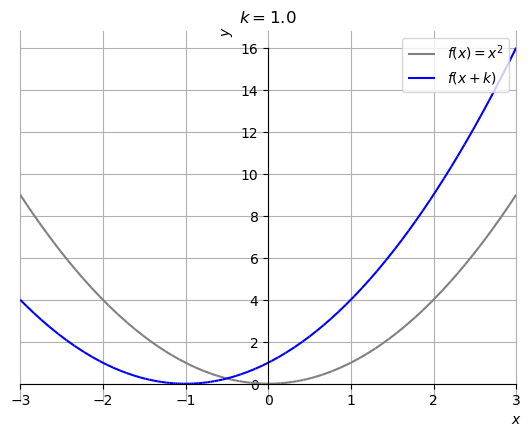
\includegraphics[width=0.6\textwidth]{fig_func/fig_ex_transhoriz}
    \caption{Esboço do gráfico de $f(x) = x^2$ e $f(x+k)$ com $k=1$.}
    \label{fig:ex_transhoriz}
  \end{figure}

  
Os comandos abaixo fazem no  \verb+GeoGebra+  os esboços dos gráficos de $f(x)$ e $f(x+k)$:
\begin{verbatim}
k = 1
f(x)=x^2
f(x+k)
\end{verbatim}
  Podemos alterar o valor de $k$ e a função $f$ para vermos o efeito das translações horizontais.
  
\end{ex}
\subsection{Dilatações e contrações}\index{Função!dilatação e contração}
Sejam dados uma função $f$ e uma constante $\alpha$. Então, o gráfico de:
\begin{itemize}
\item $y = \alpha f(x)$ é uma dilatação vertical do gráfico de $f$, quando $\alpha > 1$;
\item $y = \alpha f(x)$ é uma contração vertical do gráfico de $f$, quando $0<\alpha < 1$;
\item $y = f(\alpha x)$ é uma contração horizontal do gráfico de $f$, quando $\alpha > 1$;
\item $y = f(\alpha x)$ é uma dilatação horizontal do gráfico de $f$, quando $0<\alpha < 1$.
\end{itemize}

\begin{ex}
  Seja $f(x) = x^2$. A Figura \ref{fig:ex_dilavert}, contém os esboços dos gráficos de $f(x)$ e $\alpha\cdot f(x) = \alpha \cdot x^2$ para $\alpha = 2$.

  \begin{figure}[H]
    \centering
    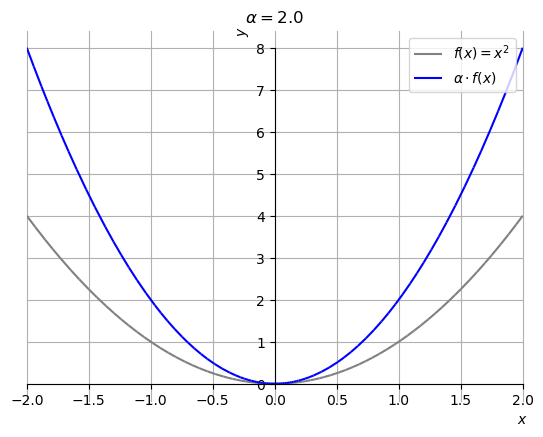
\includegraphics[width=0.6\textwidth]{fig_func/fig_ex_dilavert}
    \caption{Esboço do gráfico de $f(x) = x^2$ e $\alpha\cdot f(x)$ com $\alpha=2$.}
    \label{fig:ex_dilavert}
  \end{figure}

  
  Os seguintes comandos \verb+GeoGebra+, faz os esboços dos gráficos de $f(x)$ e $\alpha\cdot f(x)$:
\begin{verbatim}
f(x)=x^2
alpha = 2
alpha*f(x)
\end{verbatim}
  Podemos alterar o valor de \verb+alpha+ e a função \verb+f+ para vermos o efeito das dilatações/contrações verticais.
  \end{ex}

\begin{ex}
  Seja $f(x) = x^2-2x+1$. A Figura \ref{fig:ex_dilahoriz}, contém os esboços dos gráficos de $f(x)$ e $f(\alpha\cdot x) = (\alpha \cdot x)^2-2(\alpha\cdot x) + 1$ para $\alpha = \frac{1}{2}$.

  \begin{figure}[htb]
    \centering
    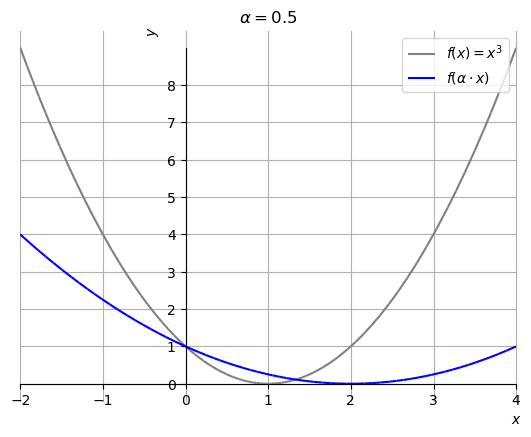
\includegraphics[width=0.6\textwidth]{fig_func/fig_ex_dilahoriz}
    \caption{Esboço do gráfico de $f(x) = x^2-2x+1$ e $f(\alpha\cdot x)$ com $\alpha=\frac{1}{2}$.}
    \label{fig:ex_dilahoriz}
  \end{figure}

    Os seguintes comandos \verb+GeoGebra+, faz os esboços dos gráficos de $f(x)$ e $f(\alpha\cdot x)$:
\begin{verbatim}
f(x) = x^2-2x+1
alpha = 2
f(alpha*x)
\end{verbatim}
  Podemos alterar o valor de \verb+alpha+ e a função \verb+f+ para vermos o efeito das dilatações/contrações horizontais.
  \end{ex}
  
\subsection{Reflexões}\index{Função!reflexão}
Seja dada uma função $f$. O gráfico da função $y = -f(x)$ é uma reflexão em torno do eixo das ordenadas do gráfico da função $f$. Já, o gráfico da função $y = f(-x)$ é uma reflexão em torno do eixo das abscissas do gráfico da função $f$.\\

\begin{ex}
  Seja $f(x) = x^2-2x+2$. A Figura \ref{fig:ex_reflex1}, contém os esboços dos gráficos de $f(x)$ e $-f(x) = -x^2+2x-2$.

  \begin{figure}[H]
    \centering
    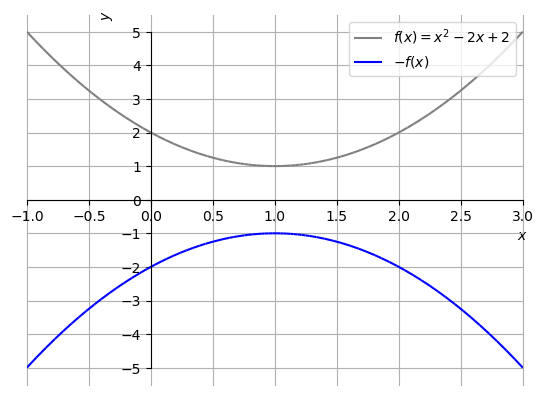
\includegraphics[width=0.63\textwidth]{fig_func/fig_ex_reflex}
    \caption{Esboço do gráfico de $f(x) = x^2-2x+2$ e $-f(x)$.}
    \label{fig:ex_reflex1}
  \end{figure}

\end{ex}

\begin{ex}
  Seja $f(x) = x^2-2x+2$. A Figura \ref{fig:ex_reflex}, contém os esboços dos gráficos de $f(x)$ e $f(-x) = x^2+2x+2$.

  \begin{figure}[H]
    \centering
    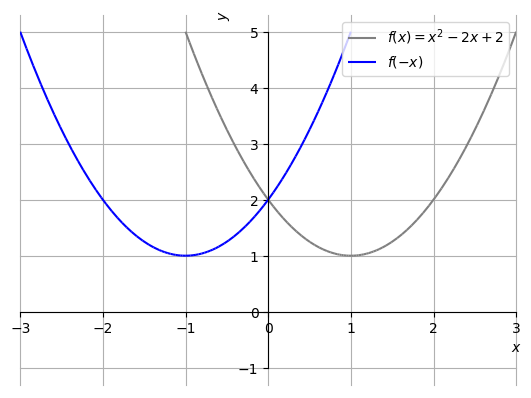
\includegraphics[width=0.63\textwidth]{fig_func/fig_ex_refley}
    \caption{Esboço do gráfico de $f(x) = x^2-2x+2$ e $f(-x)$.}
    \label{fig:ex_reflex}
  \end{figure}

  Para fazer os esboços dos gráficos de $f(x)$ e $f(-x)$ no \verb+GeoGebra+, digite:
  \begin{verbatim}
f(x) = x^2-2x+2
f(-x)
\end{verbatim}
  Podemos alterar a função \verb+f+ para vermos o efeito das reflexões em torno de eixo das ordenadas.
\end{ex}

\subsection{Exercícios resolvidos}\index{Exercícios resolvidos!operações com funções}
\begin{exeresol}
  Faça o esboço do gráfico de $f(x) = 2(x-1)^3+1$.
  \begin{resol}
  Começamos trançando o gráfico de $f_1(x) = x^3$. Então, obtemos o gráfico de $f_2(x) = (x-1)^3$ por translação de uma unidade à direita. O gráfico de $f_3(x) = 2(x-1)^3$ é obtido por dilatação vertical de 2 vezes. Por fim, o gráfico de $f_4(x) = 2(x-1)^3+1$ é obtido por translação de uma unidade para cima. Veja a Figura \ref{fig:exeresol_opfun_graf}.
  \begin{figure}[H]
    \centering
    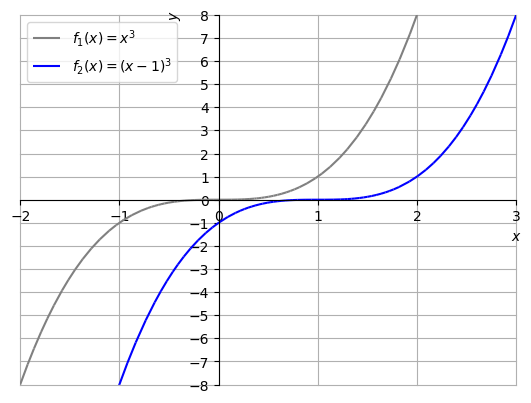
\includegraphics[width=0.49\textwidth]{fig_func/fig_exeresol_opfun_graf_1}~
    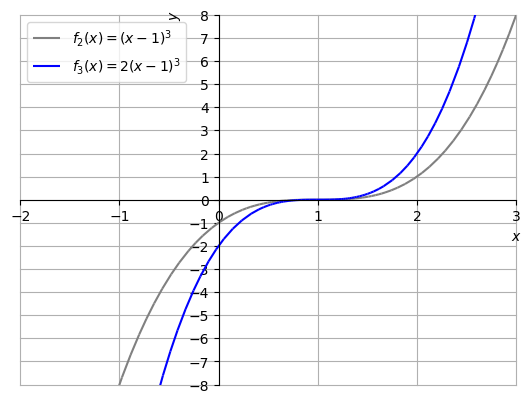
\includegraphics[width=0.49\textwidth]{fig_func/fig_exeresol_opfun_graf_2}\\
    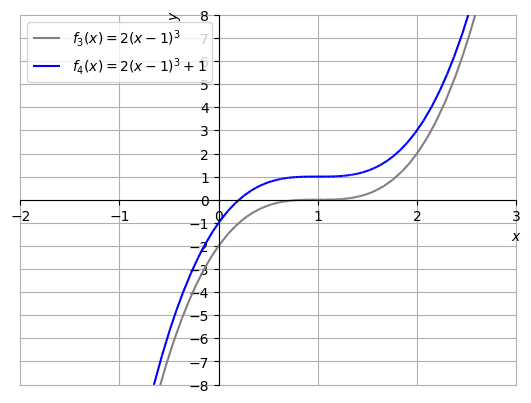
\includegraphics[width=0.49\textwidth]{fig_func/fig_exeresol_opfun_graf_3}
    \caption{Construção do esboço do gráfico de $f(x) = 2(x-1)^3+1$.}
    \label{fig:exeresol_opfun_graf}
  \end{figure}
\end{resol}
\end{exeresol}
\begin{exeresol}
  Sejam
  \begin{equation*}
    f(x) = \frac{x^2 - \sqrt{x-1}}{x}\quad\text{e}\quad g(x) = x^2 + 1.
  \end{equation*}
  Determine a função composta $(f\circ g)$ e seu domínio.
  \begin{resol}~
  Começamos determinando a função composta
  \begin{align*}
    (f\circ g)(x) &= f(g(x))\\
                  &= f(x^2 + 1)\\
                  &= \frac{(x^2 + 1)^2 - \sqrt{x^2+1-1}}{x^2 + 1}\\
                  &= \frac{x^4 + 2x^2 + 1 - \sqrt{x^2}}{x^2 + 1}\\
                  &= \frac{x^4 + 2x^2 + 1 - |x|}{x^2 + 1}
  \end{align*}
  Agora, observamos que $g$ está definida em toda parte e tem imagem $[1, \infty)$. Como o domínio da $f$ é $[1, \infty)$, temos que $(f\circ g)$ está definida em toda parte.
\end{resol}
\end{exeresol}

\subsection{Exercícios}\index{Exercícios!operações com funções}
\begin{exer}
  Sejam $f(x) = \sqrt{x}+1$ e $g(x) = x^2 -1$. Determine a função $(f\circ g)$ e seu domínio.
\end{exer}
\begin{resp}
  $(f\circ g)(x) = \sqrt{x^2-1}+1$; domínio: $(-\infty, 1]\cup [1, \infty)$.
\end{resp}

\begin{exer}
  Faça um esboço do gráfico de $g(x) = 2x^3 - 1$.
\end{exer}
\begin{resp}
  Dica: verifique sua resposta com um pacote de matemática simbólica, por exemplo, com o \geogebra.
\end{resp}

\section{Propriedades de funções}\index{Função!propriedades}\label{cap_funcao_sec_funprop}
\subsection{Funções crescentes ou decrescentes}\label{subsec:Func_Cresc-decrescentes}
\begin{framed}
\begin{definition}[Função Crescente ou decrescente]~\label{def:FuncCresc}
\\ Uma da função $f$ é dita ser crescente\index{Função!crescente} quando $f(x_1)<f(x_2)$ para todos $x_1<x_2$ no seu domínio.\\
É dita decrescente\index{Função!decrescente} quando $f(x_1)>f(x_2)$ para todo $x_1<x_2$.
\end{definition}
\end{framed}

Também, definem-se os conceitos análogos de uma função ser crescente ou decrescente em um dado intervalo.

\begin{ex}
  A função $f(x) = x^2$ é uma função decrescente no intervalo $(-\infty, 0]$ e crescente no intervalo $[0, \infty)$ (\dica Comprove!).
\end{ex}
\subsection{Funções pares ou ímpares}\label{subsec:Func_pares_impares}
\begin{framed}
\begin{definition}[Função par]~
\\ Uma dada {\bf função} $f$ é dita {\bf par}\index{Função!!par} quando $f(-x)=f(x)$ para todo $x$ no seu domínio.
\end{definition}\end{framed}
\begin{framed}
\begin{definition}[Função impar]~
\\ Uma dada {\bf função} $f$ é dita {\bf impar}\index{Função!!impar} quando $f(-x)=-f(x)$ para todo $x$ no seu domínio.
\end{definition}\end{framed}
\begin{ex}\label{ex:FuncParImpar}
  Vejamos os seguintes casos (\dica demonstre-os):
  \begin{itemize}
  \item $f(x) = x^2$ é uma função par.
  \item $f(x) = x^3$ é uma função par.
  \item $f(x) = \sen x$ é uma função ímpar.
  \item $f(x) = \cos x$ é uma função par.
  \item $f(x) = x+1$ não é par nem ímpar.
  \end{itemize}
\end{ex}

\subsection{Funções injetoras, sobrejetoras e bijetoras}\label{subsec:Func_inj_subjet_bijetoras}
\textbf{Função Injetora}

Uma função \(f:A \rightarrow B\) é dita  injetora\index{Função!injetora} (ou injetiva) quando valores diferentes no domínio geram imagens distintas no contradomínio. Ou seja, se $x_1\neq x_2$ \textbf{então} $f(x_1)\neq f(x_2)$ para todos $x_1, x_2$ no seu domínio. Equivalentemente se $f(x_1)= f(x_2)$ \textbf{então} $x_1=x_2$.\\

\textbf{Função Sobrejetora}

Uma função Função \(f:A \rightarrow B\) é dita Sobrejetora\index{Função!sobrejetora} (ou sobrejetiva) quando o contradomínio é igual à imagem, ou seja, cada elemento do contradomínio é correspondido por ao menos um do domínio: \(Imagem(f) = B\).\\

\textbf{Função bijetora}\index{Função!bijetora}

Função bijetora (ou bijetiva) é aquela que é tanto injetora como sobrejetora: \(x_1 \not= x_2 \Rightarrow f(x_1) \not= f(x_2) \mbox{ e } Imagem(f) = B\).

\begin{ex}
  Vejamos os seguintes casos:
  \begin{itemize}
  \item $f(x) = x^2$ não é uma função injetora.
  \item $f(x) = x^3$ é uma função injetora.
  \item $f(x) = e^x$ é uma função injetora.
  \end{itemize}
\end{ex}

\subsection{Exercícios resolvidos}\index{Exercícios resolvidos!propriedades das funções}
\begin{exeresol}
  Defina os intervalos em que a função $f(x) = -|x+1|$ é crescente ou decrescente.\\
  \begin{resol}
  A função $f$ é uma translação à esquerda, seguida de uma reflexão em torno do eixo das abscissas da função $f(x) = |x|$. Veja a Figura \ref{fig:exeresol_funprop_mono}.

  \begin{figure}[H]
    \centering
    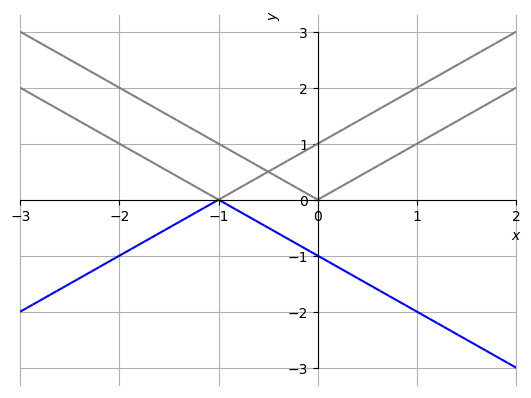
\includegraphics[width=0.6\textwidth]{fig_func/fig_exeresol_funprop_mono.png}
    \caption{Esboço do gráfico de $f(x) = -|x+1|$.}
    \label{fig:exeresol_funprop_mono}
  \end{figure}

  Do esboço do gráfico de $f$, podemos inferir que $f$ é crescente no intervalo $(-\infty, -1]$ e decrescente no intervalo $[-1, \infty)$.
\end{resol}
\end{exeresol}
\begin{exeresol}
  Analise a paridade da função $tg(x)$.
  \begin{resol}
  Da paridade das funções seno e cosseno, temos
  \begin{equation}
    \tg(-x) = \frac{\sen(-x)}{\cos(-x)} = \frac{-\sen x}{\cos x} = -\frac{\sen x}{\cos x} = -\tg x
  \end{equation}
  Logo, a tangente é uma função ímpar.
\end{resol}
\end{exeresol}
\begin{exeresol}
  Calcule a função inversa de $f(x) = \sqrt{x+1}$.
  \begin{resol}
  Para obtermos a função inversa de uma função $f$, resolvemos $y = f(x)$ para $x$. Ou seja,
  \begin{align*}
    y = f(x) &\Rightarrow y = \sqrt{x+1}\\
             &\Rightarrow y^2 = x+1\\
             &\Rightarrow x = y^2 - 1
  \end{align*}
  Logo, temos $f^{-1}(x) = x^2 - 1$ restrita ao conjunto imagem da $f$, i.e. o domínio de $f^{-1}$ é $[0, \infty)$.
\end{resol}
\end{exeresol}

\subsection{Exercícios}\index{Exercícios!propriedades das funções}
\begin{exer}
  Comprove que as funções do Exemplo \ref{ex:FuncParImpar} são par ou impar, conforme o caso, utilizando as definições dadas.
\end{exer}

\begin{exer}
  Determine os intervalos de crescimento ou decrescimento da função
  \begin{equation}
    f(x) = \left\{
      \begin{array}{ll}
        (x+1)^2, & -\infty < x \leq 1\\
        -x+5, & 1 \leq x < \infty
      \end{array}
\right.
  \end{equation}
\end{exer}
\begin{resp}
  decrescente: $(-\infty, -1]\cup [1, \infty)$; crescente: $[-1, 1]$.
\end{resp}

\begin{exer}
  Analise a paridade da função $\cosec x$.
\end{exer}
\begin{resp}
  função ímpar
\end{resp}

\begin{exer}
  Seja $f(x) = 2\sqrt{x-1}-1$. Calcule $f^{-1}$ e determine seu domínio.
\end{exer}
\begin{resp}
  $f^{-1}(x) = \frac{1}{2}x^2 + x - \frac{1}{2}$; domínio $[-1, \infty)$
\end{resp}

\section{Funções exponenciais}\index{Função!exponencial}\label{sec:Exponencial}
\subsection{Definição e exemplos}\index{Exponencial!definição e exemplos}
Uma {\bf função exponencial}\index{Função!!exponencial} tem a forma
\begin{equation}
  f(x) = a^x
\end{equation}
onde $a\neq 1$ é uma constante positiva e é chamada de {\bf base}\index{base} da função exponencial.

Funções exponenciais estão definidas em toda parte e têm imagem $(0, \infty)$. O gráfico de uma função exponencial sempre contém os pontos $(-1,1/a)$, $(0,1)$ e $(1,a)$. Veja a Figura \ref{fig:GrafExp}.

Quando $a>1$ a função é crescente e quando $0<a<1$ é decrescente. O gráfico da esquerda na Figura \ref{fig:GrafExp} exemplifica uma função crescente e da direita, decrescente.
\begin{figure}[H]
  \centering
  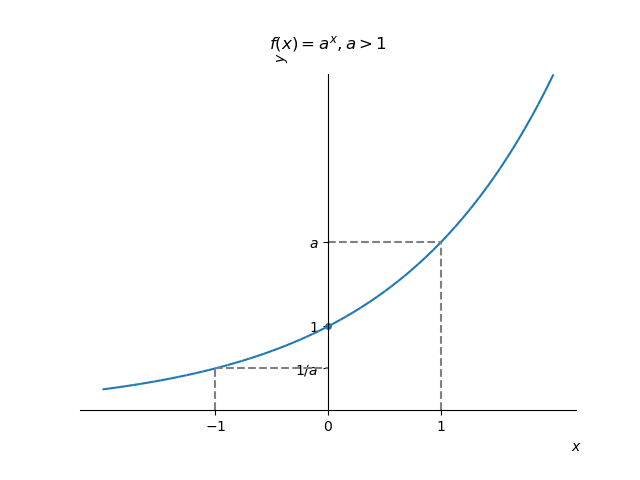
\includegraphics[width=0.5\textwidth]{fig_func/fig_exponencial_2}~
  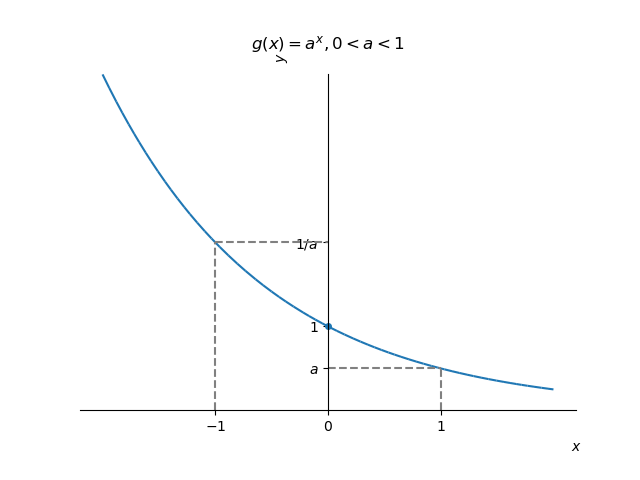
\includegraphics[width=0.5\textwidth]{fig_func/fig_exponencial_12}
  \caption{Esboços dos gráficos de funções exponenciais: (esquerda) $f(x) = a^x$, $a>1$; (direita) $g(x) = a^x$, $0<a<1$.}
  \label{fig:GrafExp}
\end{figure}

\begin{ex}~
\pichskip{0.5cm}%distância entre texto e figura
\parpic(4.9cm,4.9cm)(0cm,3.2cm)[r]{%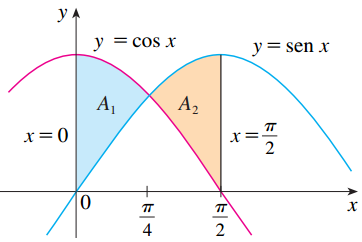
\includegraphics[scale=0.75]{cap_apl_integracao/figs/AreaEntreFuncSenCos.png}}
\begin{minipage}{0.45\textwidth}
\includegraphics[scale=1.1]{fig_func/ExFuncTabXadrez}
\vspace{-0.3cm}
\captionof*{figure}{\footnotesize{Ilustração da ``Recompensa de\\ Sessa'', um conto de Malba Tahan,\\ do livro Lendas do oásis.}}
\label{fig:xadrez}
\end{minipage}
}
\noindent Para ilustrar o conceito de função exponencial, recorremos ao exemplo, narrado no livro de Malba Tahan, do Marajá, que a fim de saldar uma dívida concordou em fazer o pagamento a Sessa (um dos seus súditos) da seguinte maneira: \textit{no primeiro ano, o súdito  receberia apenas um grão de trigo.  No segundo ano, ele receberia  míseros dois grãos de trigo, duplicando daí em diante, a cada ano, o  número de grãos até a última casa do tabuleiro de xadrez.}

\noindent Assim,  o número de grãos $N$ seria dado em função do número de anos $n$ e expresso pela fórmula:
$$ N=2^n $$
\vspace{0.1cm}

O súdito elaborou a Tabela \ref{tab:Graos}, baseada em uns poucos anos
%\vspace{-0.2cm}
\begin{table}[htb]
    \centering
    \begin{tabular}{|c|c|c|c|c|c|c|c|}
    \hline
\rowcolor{cyan}\cellcolor{blue}   Número de anos &1& 2& 3& 4& 5& 6& 7\\\hline
\rowcolor{magenta}\cellcolor{red} Número de grãos de trigo&  2 &4 &8& 16& 32 &64 &128\\\hline
             \end{tabular}
    \caption{Número de grãos a cada ano, até o sétimo ano.}
    \label{tab:Graos}
\end{table}
\begin{center}
\fbox{\parbox{9cm}{\center{\blu{Para Pensar!}\\
\vspace{0.2cm}
Quantos grãos seriam depois de 20 anos? \\
E depois de 40?}
}}\end{center}

Depois de 8 anos, deveria depositar na última casa da primeira fileira do tabuleiro apenas 256 grãos.
 
Uma bagatela, portanto.  Não entendendo de funções  exponenciais, o soberano aceitou, para sua desgraça, essa forma de pagamento.

\desafio{Quantos grãos de trigo Sessa receberá do Marajá?}
\end{ex}


\begin{comment}

\begin{figure}[H]
\begin{ex}~
\\ \begin{minipage}{0.65\linewidth}
Para ilustrar o conceito de função exponencial, recorremos ao exemplo, narrado no livro de Malba Tahan, do Marajá, que a fim de saldar uma dívida concordou em fazer o pagamento a Sessa (um dos seus súditos) da seguinte maneira: \textit{no primeiro ano, o súdito  receberia apenas um grão de trigo.  No segundo ano, ele receberia  míseros dois grãos de trigo, duplicando daí em diante, a cada ano, o  número de grãos até a última casa do tabuleiro de xadrez.}
\end{minipage}\hfill
\begin{minipage}{0.32\linewidth}
 \includegraphics{1-cap_func/fig_func/ExFuncTabXadrez}
 \vspace{-0.4cm}
\caption*{\scriptsize{Ilustração da ``Recompensa de Sessa'', um conto de Malba Tahan, do livro Lendas do oásis.}}

\end{minipage}
\bigskip
Assim,  o número de grãos $N$ seria dado em função do número de anos $n$ e expresso pela fórmula
\begin{equation}
  N=2^n 
\end{equation}

O súdito elaborou a Tabela 6.2, baseada em uns poucos anos:
\begin{table}[H]
    \centering
    \begin{tabular}{|c|c|c|c|c|c|c|c|}
    \hline
\rowcolor{cyan}\cellcolor{blue}   Número de anos &1& 2& 3& 4& 5& 6& 7\\\hline
\rowcolor{magenta}\cellcolor{red} Número de grãos de trigo&  2 &4 &8& 16& 32 &64 &128\\\hline
             \end{tabular}
    \caption{Número de grãos a cada ano, até o sétimo ano.}
    \label{tab:Graos}
\end{table}
\begin{center}
\fbox{\parbox{9cm}{\center{\blu{Para Pensar!}\\
\vspace{0.2cm}
Quantos grãos seriam depois de 20 anos? \\
E depois de 40?}
}}\end{center}


 Depois de 8 anos, deveria depositar na última casa da primeira fileira do tabuleiro apenas 256 grãos.
 
Uma bagatela, portanto.  Não entendendo de funções  exponenciais, o soberano aceitou, para sua desgraça, essa forma de pagamento.\\
\desafio{Quantos grãos de trigo Sessa receberá do Marajá?}
\end{ex}
\end{figure}

\end{comment}


A função exponencial mais importante entre todas, do ponto de vista científico, é a função exponencial que tem como base o número $e\approx 2,718281828459045$, conhecido como número de Euler\footnote{Acesse informações sobre o número $e$ \href{https://waldexifba.wordpress.com/2015/12/23/onumeroe/}{neste post em waldexifba.}}. Esse número, assim como o número $\pi$, é um dos números mais importantes das ciências.

Um bom exemplo da relevância da função exponencial de base e diz respeito ao decaimento 
de substâncias radioativas.  Nesse caso, o número de átomos $N$ que compõem uma determinada 
substância varia com o tempo ($t$) de acordo com a expressão
\begin{equation}
    N=N_0e^{-\lambda t}
\end{equation}
onde $N_ 0$ é o número de átomos presentes no instante de tempo $t = 0$ e $\lambda$ é uma constante característica do material, que recebe o nome de constante radioativa.

Definimos ainda funções exponenciais especiais considerando combinações de funções 
exponenciais.  Por exemplo, definimos as funções: seno hiperbólico e cosseno hiperbólico como aquelas dadas pelas combinações:
\begin{equation}
    \sinh=\frac{e^x-e^{-x}}{2}\quad\textrm{ e  } \quad \cosh=\frac{e^x+e^{-x}}{2}
\end{equation}
\subsection{Exercícios resolvidos}\index{Exercícios resolvidos!exponencial}
\begin{exeresol}
  Faça um esboço do gráfico de $f(x) = e^{-2x+1}-1$.
\end{exeresol}
\begin{resol}
Primeiramente, observamos que $f(x) = e^{-2x+1}-1 = e^{-2\left(x-\frac{1}{2}\right)}-1$. Então, partindo do gráfico de $e^{-x}$, fazemos uma translação de $1/2$ unidades à direita, seguida de uma contração horizontal de $1/2$ vezes e, por fim, uma translação para baixo de uma unidade. Veja a Figura \ref{fig:exeresol_funexp_graf}.

  \begin{figure}[htb]
    \centering
    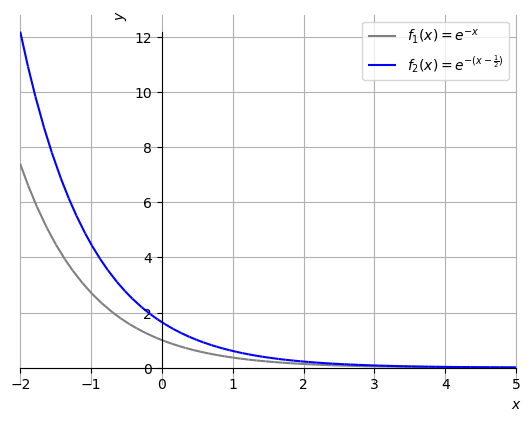
\includegraphics[width=0.49\textwidth]{fig_func/fig_exeresol_funexp_graf_1}~
    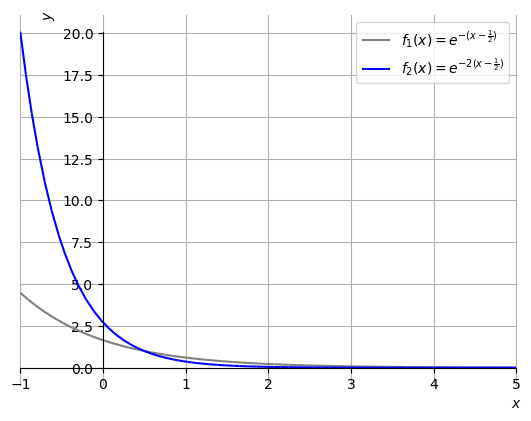
\includegraphics[width=0.49\textwidth]{fig_func/fig_exeresol_funexp_graf_2}\\
    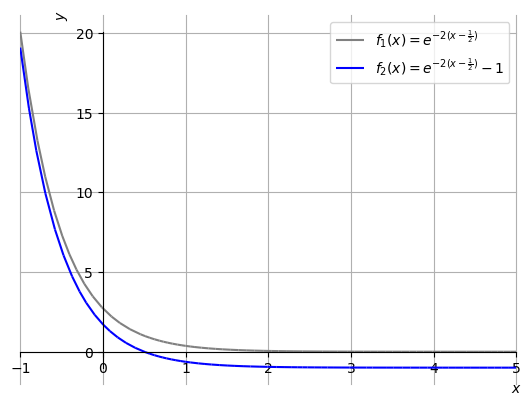
\includegraphics[width=0.49\textwidth]{fig_func/fig_exeresol_funexp_graf_3}
    \caption{Esboço do gráfico de $f(x) = e^{-2x+1}-1$.}
    \label{fig:exeresol_funexp_graf}
  \end{figure}
\end{resol}

\section{Funções logarítmicas}\index{Função!logarítmica}\label{sec:logaritmo}
\subsection{Definição}\index{Logaritmo!definição}
A {\bf função logarítmica}\index{Função!!logarítmica} $\boldsymbol{y = \log_a x}$, $a>0$ e $a\neq 1$, é a função inversa da função exponencial $y = a^x$. Veja a Figura \ref{fig:log_graficos}. O domínio da função logarítmica é $(0,\infty)$ e a imagem $(-\infty, \infty)$.

\begin{figure}[hbt]
  \centering
  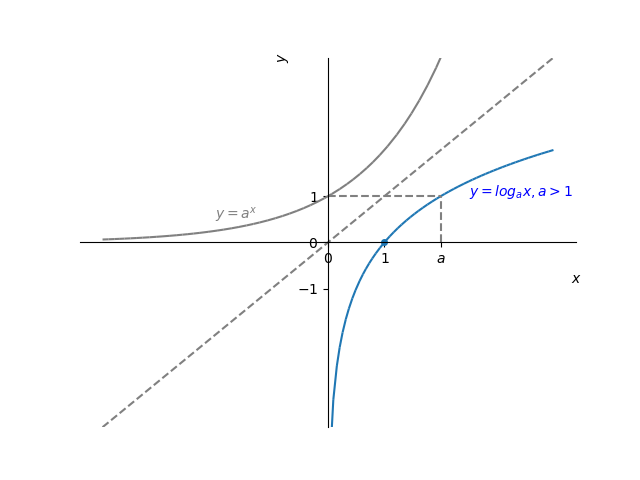
\includegraphics[width=0.5\textwidth]{fig_func/fig_log_2}~
  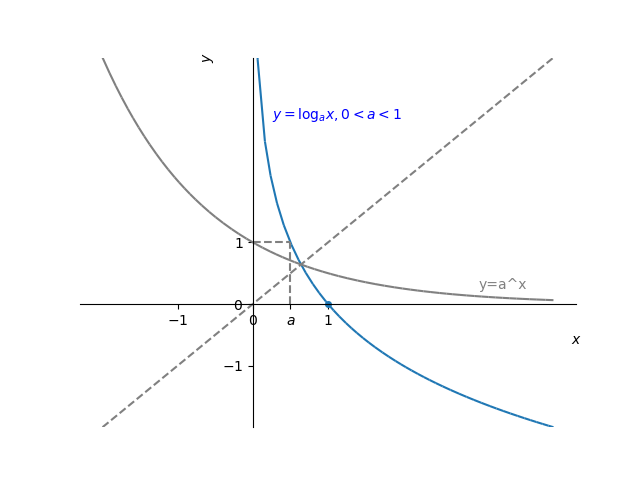
\includegraphics[width=0.5\textwidth]{fig_func/fig_log_12}
  \caption{Esboços dos gráficos de funções logarítmicas: (esquerda) $y = \log_a x$, $a>1$; (direita) $y = \log_a x$, $0<a<1$.}
  \label{fig:log_graficos}
\end{figure}

\nota{
  Quando a base é o número de Euler $e \approx 2,718281828459045$, chamamos $y = \log_e x$ de função exponencial natural e denotamo-la por $y = \ln x$. 
}
\newpage
\subsection{Propriedades dos Logaritmos}\index{Logaritmo!propriedades}

  Vejamos algumas propriedades dos logaritmos:
  \begin{compactenum}[a.]
  \begin{multicols}{2}
  \item $\displaystyle \log_a x = y \Leftrightarrow a^y = x$
  \item $\displaystyle \log_a 1 = 0$
  \item $\displaystyle \log_a a = 1$
  \item $\displaystyle \log_a a^x = x$
   \item $\displaystyle a^{\log_a^x} = x$
    \end{multicols}
  \item $\displaystyle \log_a xy = \log_a x + \log_a y$ (\textit{Logaritmo do produto});\\
  \item $\displaystyle \log_a \frac{x}{y} = \log_a x - \log_a y$ (\textit{Logaritmo do quociente});
  \item $\displaystyle \log_a x^r = r\cdot\log_a x$ (\textit{Logaritmo da potência}).
  \item $\displaystyle \log_a x = \frac{\log_b x}{\log_b a}$ (\textit{Mudança de base}).
  \end{compactenum}
\subsection{Exercícios resolvidos}\index{Exercícios resolvidos!logaritmo}
\begin{exeresol}
  Faça o esboço do gráfico de $f(x) = \ln(x+2)+1$ e determine seu domínio.
  \begin{resol}
  Para fazermos o esboço do gráfico de $f(x) = \ln(x+2)+1$, podemos começar com o gráfico de $f_1(x) = \ln x$. Então, podemos transladá-lo 2 unidades à esquerda, de forma a obtermos $f_2(x) = \ln(x+2) = f_1(x+2)$. Por fim, transladamos o gráfico de $f_2(x)$ uma unidade para cima, obtendo o esboço do gráfico de $f(x) = \ln(x+2)+1=f_2(x)+1$. Veja a Figura \ref{fig:exeresol_lograf}.

  \begin{figure}[H]
    \centering
    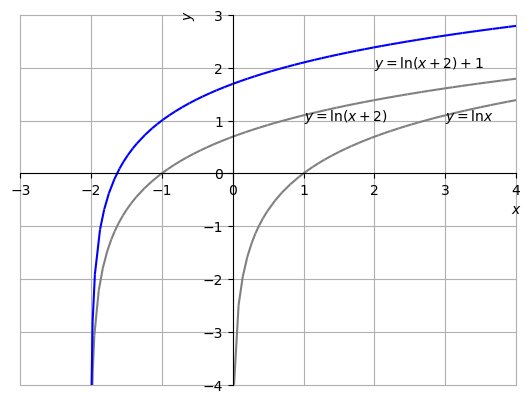
\includegraphics[width=0.5\textwidth]{fig_func/fig_exeresol_lograf}
    \caption{Esboço do gráfico de $f(x) = \ln(x+2)+1$.}
    \label{fig:exeresol_lograf}
  \end{figure}

Ainda, o domínio de $\ln x$ é $(0, \infty)$. Como, $f(x) = \ln(x+2)+1$ é uma translação de duas unidades à esquerda e uma para cima de $\ln x$, temos que o domínio de $f(x)$ é $(-2, \infty)$.
\end{resol}
\end{exeresol}
\begin{exeresol}
  Resolva a seguinte equação para $x$
  \begin{equation}
    \ln(x+2) + 1 = 1
  \end{equation}
  \begin{solution}
  Podemos calcular a solução pelos seguintes passos:
  \begin{align*}
    \ln(x+2)+1=1 &\Rightarrow \ln(x+2)=0\\
                 &\Rightarrow x+2=e^0\\
                 &\Rightarrow x=1-2=-1\\
  \end{align*}

  Com o \geogebra, podemos computar a solução com o seguinte comando:
\begin{verbatim}
Resolver(ln(x+2)+1=1)
\end{verbatim}
\end{solution}
\end{exeresol}

\subsection{Exercícios}\index{Exercícios!logaritmo}

\begin{exer}
  Faça o esboço do gráfico de $f(x) = \log(x-2)-1$ e determine seu domínio.
\end{exer}
\begin{resp}
  Dica: use um pacote computacional de matemática simbólica para verificar o esboço de seu gráfico. Domínio: $(2, \infty)$.
\end{resp}

\begin{exer}
  Resolva a seguinte equação para $x$
  \begin{equation*}
    \ln(x+1)^2=0
  \end{equation*}
\end{exer}
\begin{resp}
  $0$
\end{resp}
\begin{exer}
Suponha que uma substância radioativa se desintegre, de modo que, partindo de uma quantidade $Q_0$, a quantidade existente após $t$ anos seja dada por $Q(t) = Q_0 e^{-0,05t}$.. Dado $\ln 2 = 0,693$, calcule $t$ de modo que se tenha $Q(t) = 0,5 Q_0$, isto é, encontre a meia-vida dessa substância, e marque a alternativa correspondente.
\begin{multicols}{3}
\begin{compactenum}[a)]
\item  Cerca de 8 anos\item  Cerca de 10 anos\item Cerca de 12 anos\item Cerca de 14 anos\item Cerca de 16 anos.
\end{compactenum}
\end{multicols}
\end{exer}
\begin{resp}
d
\end{resp}
\begin{exer}
Em certa cultura de bactérias, verificou-se que a população está se reproduzindo e aumentando seu número em 25\% a cada dia. Determine o número aproximado de dias que devem se passar para que o número de bactérias seja 200 vezes maior que o número inicial.\\
Use as aproximações $\log 2 = 0,301$ e $\log 5 = 0,699$.
\begin{multicols}{3}
\begin{compactenum}[a)]
\item 18 dias\item 24 dias\item  36 dias\item  48 dias\item  60 dias
\end{compactenum}
\end{multicols}
\end{exer}
\begin{resp}
b
\end{resp}
\begin{exer}
(Unicamp) O álcool no sangue de um motorista alcançou o nível de 2 gramas por litro logo depois de ele ter bebido uma considerável quantidade de vodca. Considere que esse nível decresce de acordo com a fórmula $N(t) = 2\cdot (0,5)^t$, em que $t$ é o tempo medido em horas a partir do momento em que o nível é constatado. Quanto tempo deverá o motorista esperar, antes de dirigir seu veículo, se o limite permitido de álcool no sangue, no país em que ele se encontra, é de $0,8$ grama por litro? (Use $\log 2 = 0,3$)
\begin{multicols}{3}
\begin{compactenum}[a)]
\item 4/3 hora\item  1 hora e meia\item  5/3 hora\item  2 horas\item 2 horas e meia
\end{compactenum}
\end{multicols}
\end{exer}
\begin{resp}
a
\end{resp}

\section{Alguns exemplos de aplicações}\index{Função!aplicações}\label{sec:Func-Aplicacoes}
O conceito de função é importante na física e em outras áreas do conhecimento porque muitas vezes uma grandeza física,  $y$, depende de outra ou outras, usualmente o tempo ou as coordenadas. No caso de apenas uma variável independente representaremos tal dependência da seguinte forma:
\matt{
y=f(x)
}
que se lê  $y$ é função de  $x$.

Na mecânica, a variável independente é o tempo. As variáveis que podem depender do 
tempo são as coordenadas, a velocidade, a aceleração e, em alguns casos, a própria força.

Nos exemplos abaixo, tanto o domínio da função quanto o contradomínio são o conjunto $\mathbb{R}$,  

\subsection{Área de um quadrado}
\pichskip{0.1cm}%distância entre texto e figura
\parpic(4.5cm,3.5cm)(-0.1cm,2.3cm)[r]{%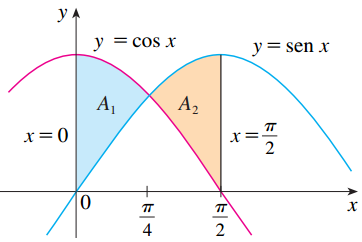
\includegraphics[scale=0.75]{cap_apl_integracao/figs/AreaEntreFuncSenCos.png}}
\begin{minipage}{0.25\textwidth}
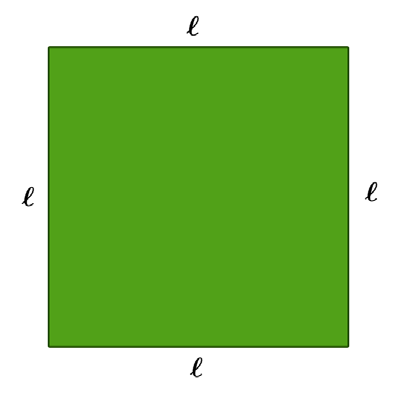
\includegraphics[scale=0.45]{fig_func/quadrado}
\vspace{-0.9cm}
\captionof{figure}{}%
\label{fig:AreaQuadrado}
\end{minipage}
}
\noindent O primeiro exemplo a ser considerado vem da geometria. A área $A$ de um quadrado depende do comprimento de um dos seus lado. Se $l$ representa esse comprimento, conforme Figura \ref{fig:AreaQuadrado}, essa dependência se escreve:
\matt{
A=l^2
}
\vspace{1cm}
\subsection{Força Elástica}
\figtext{0.5cm}{r}{0.3}{%
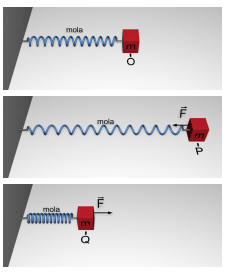
\includegraphics[width=4.6cm]{fig_func/MolaElastica}
\captionof{figure}{}
\label{fig:ExForcaElast}
}%
\noindent\ Um exemplo simples da mecânica ilustra o conceito de função. Trata-se de um exemplo envolvendo uma dependência linear entre grandezas. Consideremos um corpo de massa $m$ que esteja apoiado num plano horizontal e preso na extremidade de uma mola. Consideremos ainda o caso em que a outra extremidade da mola esteja fixada numa parede vertical sem que haja qualquer tipo de interferência no sistema massa-mola, o conjunto permanecerá em repouso. E isto ocorre quando a mola não está sujeita  a nenhuma deformação.

\noindent Se, no entanto, esticarmos ou comprimirmos a mola (puxando ou empurrando o corpo até uma nova posição), conforme ilustrado na Figura \ref{fig:ExForcaElast} vamos notar que ela exerce uma força, $F$, sobre o corpo de massa $m$. Essa força, denominada força elástica age de forma a restaurar a posição original, a posição de equilíbrio. Se adotarmos a convenção de que a origem da coordenada associada ao deslocamento coincida com o ponto no qual não existem forças sobre a mola (a posição de equilíbrio), podemos 
escrever a dependência da força em relação à coordenada da seguinte forma:
\matt{
F=-kx
}
onde $k$ é uma constante denominada \textbf{constante elástica da mola}. Observe que, se aumentarmos o valor do deslocamento, em módulo, a força aumentará. O sinal menos assegura que ela está sempre no sentido do ponto de equilíbrio. Nesse ponto, a força é nula.
\subsection{Gravitação}
\pichskip{0.5cm}%distância entre texto e figura
\parpic(5.5cm,4.5cm)(-0.1cm,2.3cm)[r]{%\includegraphics[scale=0.75]{cap_apl_integracao/figs/AreaEntreFuncSenCos.png}}
\begin{minipage}{0.3\textwidth}
\includegraphics[scale=0.2]{fig_func/Gravitação}
\vspace{-0.9cm}
\captionof{figure}{}%
\label{fig:ExGravitação}
\end{minipage}
}
\noindent Um exemplo extraído da gravitação diz respeito ao tempo de queda de um corpo, uma 
vez solto de uma altura $h$. Tal tempo depende da aceleração da gravidade e depende da raiz 
quadrada da altura. O tempo de queda pode ser visto como dependente desses dois parâmetros. 

\noindent Visto como dependente da altura, escrevemos essa dependência como a função:\\
\matt{
T_{queda}=\sqrt{\frac{2}{g}}\sqrt{h}
}
\noindent O gráfico dessa função, para diferentes valores da altura, é representado na \mbox{Fig. \ref{fig:ExGravitação}.} 
\section{Recapitulando}\index{Recapitulando!funções}
Neste capítulo, apresentamos o importante conceito de função com o intuito de fazer com que o aluno determine com precisão o domínio, a imagem e o gráfico de uma função real dada; estes conceitos também foram abordados e foram apresentados diversos exemplos ilustrando esses tópicos.

Nas seções subsequentes, apresentamos alguns casos particulares de funções, com as quais vamos a lidar no decorrer deste livro, assim como as operações aritméticas e composições que as envolvem. Por último, e não menos importante, a teoria sobre a inversa de uma função foi apresentada.

Um tratamento especial foi dado as funções afim (seção \ref{sec:FuncAfim}), quadrática (seção \ref{sec:FuncQuadratica}), exponencial (seção \ref{sec:Exponencial}), logarítmica (seção \ref{sec:logaritmo}) e as funções trigonométricas seno, cosseno, tangente, cotangente, secante e cossecante (seção \ref{sec:FuncTrigonometricas}).

No próximo capítulo, apresentaremos as noções básicas sobre limites, o qual nos permitirá definir com precisão a noção de continuidade, a qual é uma das ideias mais importantes e mais fascinantes de toda a matemática.
\end{document}